% concatenated from main.tex
\documentclass[12pt]{amsart}

\usepackage[utf8]{inputenc}

\usepackage{natbib}
%\usepackage[
%  backend=biber,
%  style=authoryear,    % mimics plainnat
%  natbib=true,    % so \citep/\citet still work
%  doi=false,
%  url=false,
%  isbn=false
%]{biblatex}


%\addbibresource{Glasso-20221101.bib}

\usepackage{orcidlink}
%\usepackage[notref,notcite]{showkeys}%shows labels when editing


\usepackage{amsmath,amstext,amssymb,amsopn,amsthm}
\usepackage{url,verbatim}
\usepackage{mathtools}
\usepackage{enumerate}


\usepackage{breqn}

\usepackage{color,graphicx}

\usepackage[margin=30mm]{geometry}

\allowdisplaybreaks



\usepackage{hyperref}
\usepackage{epstopdf}

\numberwithin{equation}{section}


\usepackage{tikz}
\usetikzlibrary{decorations.pathreplacing}
\usetikzlibrary{intersections,calc,arrows.meta,patterns}

 \usepackage{booktabs}

\makeatletter
\g@addto@macro\th@plain{\thm@headpunct{}}
\makeatother

\numberwithin{equation}{section}


\newtheorem{thm}{Theorem}[section]
\newtheorem*{thm*}{Theorem}
\newtheorem{lemma}[thm]{Lemma}
\newtheorem{Corollary}[thm]{Corollary}
\newtheorem{proposition}[thm]{Proposition}

\theoremstyle{definition}
\newtheorem{conj}[thm]{Conjecture}
\newtheorem{defin}[thm]{Definition}
\newtheorem{problem}[thm]{Problem}
\newtheorem{remark}[thm]{Remark}
\newtheorem{example}[thm]{Example}

\newcommand{\R}{\mathbb{R}}
\renewcommand{\P}{\mathbb{P}}
\newcommand{\N}{\mathbb{N}}
\newcommand{\Q}{\mathrm{Q}_{\Mast}}
\newcommand{\Z}{\mathbb{Z}}
\newcommand{\E}{\mathbb{E}}
\newcommand{\I}{\mathrm{I}}

\newcommand{\cH}{\eta}

\newcommand{\norm}{\,\mathrm{pen}}
\newcommand{\normd}{\,\mathrm{pen}^\ast}
\newcommand{\norms}{\,\mathrm{pen}_{\mathcal{M}^\ast}}
\newcommand{\normsd}{\,\mathrm{pen}_{\mathcal{M}^\ast}^\ast}
\newcommand{\poly}[1]{\left\|#1\right\|_\diamond}
\newcommand{\polyd}[1]{\left\|#1\right\|^\ast_\diamond}
\newcommand{\polydr}[2]{\left\|#1\right\|^\ast_{\diamond\mid #2}}
\newcommand{\proj}{\mathrm{\mathbf{P}}_{\mathcal{M}^\ast}}
\newcommand{\PM}{\mathrm{P}_{\mathcal{M}^\ast}}
\newcommand{\PMp}{\mathrm{P}^+_{\mathcal{S}^\ast}}
\newcommand{\PP}{\mathrm{P}}
\newcommand{\Sast}{\mathcal{S}^\ast}
\newcommand{\Mast}{\mathcal{M}^\ast}
\renewcommand{\SS}{\mathcal{S}}

\newcommand{\cnorm}[1]{[\mkern-1.5mu[#1]\mkern-1.5mu]}

\DeclareMathOperator*{\argmin}{\arg\min}
\DeclareMathOperator*{\argmax}{\arg\max}
\newcommand{\tr}[1]{\mathrm{tr}\left(#1\right)}
\renewcommand{\v}[1]{\mathrm{vec}(#1)}
\newcommand{\vp}[1]{\mathrm{vec_+}(#1)}
\newcommand{\patt}[1]{\mathrm{patt}_{\diamond}\!\left(#1\right)}
\newcommand{\scalar}[2]{\left\langle\,#1\,\middle|\,#2\,\right\rangle}



\makeatletter
\newcommand{\opnorm}{\@ifstar\@opnorms\@opnorm}
\newcommand{\@opnorms}[1]{%
	\left|\mkern-1.5mu\left|\mkern-1.5mu\left|
	#1
	\right|\mkern-1.5mu\right|\mkern-1.5mu\right|
}
\newcommand{\@opnorm}[2][]{%
	\mathopen{#1|\mkern-1.5mu#1|\mkern-1.5mu#1|}
	#2
	\mathclose{#1|\mkern-1.5mu#1|\mkern-1.5mu#1|}
}
\makeatother


\makeatletter
\newcommand{\copnorm}{\@ifstar\@copnorms\@copnorm}
\newcommand{\@copnorms}[1]{%
\left|\mkern-1.5mu\left|\mkern-1.5mu\left|
	#1
\right|\mkern-1.5mu\right|\mkern-1.5mu\right|
}

\newcommand{\@copnorm}[2][]{%
	\mathopen{#1[\mkern-1.5mu#1[\mkern-1.5mu#1[}
	#2
	\mathclose{#1]\mkern-1.5mu#1]\mkern-1.5mu#1]}
}
\makeatother


\newcommand{\Set}[2]{\left\{#1;\,#2\right\}}

\title[From Graphical Lasso to Atomic Norms]{From Graphical Lasso to Atomic Norms: High-Dimensional Pattern Recovery}
%vs\\
%Pattern Recovery in High-Dimensional Precision Matrix Estimation via Atomic Norms}

%

\author[P. Graczyk]{Piotr Graczyk}
\email{piotr.graczyk@univ-angers.fr}
\address{Univ Angers, CNRS, LAREMA, SFR MATHSTIC, F-49000 Angers, France}
\address{Faculty of Pure and Applied Mathematics, Wrocław University of Science and Technology, Wybrzeże Wyspiańskiego 27, 50-370 Wroc\l{}aw, Poland}
\author[B. Kołodziejek]{Bartosz Kołodziejek \orcidlink{0000-0002-5220-9012}}
\email{bartosz.kolodziejek@pw.edu.pl}
\address{Faculty of Mathematics and Information Sciences, Warsaw University of Technology, Koszykowa 75, \mbox{00-662} Warsaw, Poland}
\author[H. Nakashima]{Hideto Nakashima}
\email{h-nakashima@tokai.ac.jp}
\address{Department of Mathematics, Faculty of Science, Tokai University, 4-1-1, Kitakaname, Hiratsuka, Kanagawa, 259-1292, Japan}

\author[M. Wilczyński]{Maciej Wilczyński}
\email{maciej.wilczynski@pwr.edu.pl}
\address{Faculty of Pure and Applied Mathematics, Wrocław University of Science and Technology, Wybrzeże Wyspiańskiego 27, 50-370 Wroc\l{}aw, Poland}

\thanks{For the purpose of Open Access, the authors have applied a CC-BY public copyright licence to any Author Accepted Manuscript (AAM) version arising from this submission.
}
\begin{document}



\begin{abstract}
Estimating high-dimensional precision matrices is a fundamental problem in modern statistics, with the graphical lasso and its $\ell_1$-penalty being a standard approach for recovering sparsity patterns. However, many statistical models, e.g. colored graphical models, exhibit richer structures like symmetry or equality constraints, which the $\ell_1$-norm cannot adequately capture. This paper addresses the gap by extending the high-dimensional analysis of pattern recovery to a general class of atomic norm penalties, particularly those whose unit balls are polytopes, where patterns correspond to the polytope's facial structure. We establish theoretical guarantees for recovering the true pattern induced by these general atomic norms in precision matrix estimation. 

Our framework builds upon and refines the primal-dual witness methodology of Ravikumar et al. (2011). Our analysis provides conditions on the deviation between sample and true covariance matrices for successful pattern recovery, given a novel, generalized irrepresentability condition applicable to any atomic norm. When specialized to the $\ell_1$-penalty, our results offer improved conditions---including weaker deviation requirements and a less restrictive irrepresentability condition---leading to tighter bounds and better asymptotic performance than prior work. The proposed general irrepresentability condition, based on a new thresholding concept, provides a unified perspective on model selection consistency. Numerical examples demonstrate the tightness of the derived theoretical bounds.
\end{abstract}

\subjclass[2020]{Primary 62F12; secondary 62H22}


\maketitle
\smallskip
\noindent \textbf{Keywords.} Precision matrix, pattern, sparsity, colored graphical models, regularization, atomic norms


\section{Introduction}

Estimating high-dimensional precision matrices is a central problem in modern statistics. Graphical models provide a powerful framework for uncovering conditional-independence structures.  \citet{Ravi2008, ravikumar2011graphical} made seminal contributions by analyzing the graphical LASSO (GLASSO) estimator \citep{YuanLi07, glasso3, Friedman2008}, focusing on its ability to recover both the support and the sign pattern of the true precision matrix. The GLASSO employs a standard $\ell_1$-penalty and is tailored to exploit simple sparsity.

Many statistical models, however---most notably colored graphical models---exhibit richer structure, such as symmetry or equality constraints among precision-matrix entries. Colored Gaussian graphical models, introduced by \citet{HL08}, combine two complementary forms of parsimony: sparsity induced by conditional independence zeros and symmetry imposed via equality constraints on entries. Recovering these structures requires penalties beyond the $\ell_1$-norm.


To capture more elaborate patterns, alternative regularizers have been proposed. The $\ell_\infty$-norm, for example, can isolate a cluster of entries with the largest magnitudes \citep{ellinfty}. The SLOPE/OWL norm \citep{Negrinho, bogdan2015slope, figueiredo16} offers a more sophisticated approach, interpolating between $\ell_1$ and $\ell_\infty$ properties. Its induced patterns can include sparsity (support), multiple clusters of equal-valued entries, and hierarchical relationships between these clusters \citep{schneider2020geometry,7aut}. Consequently, penalties like SLOPE appear well-suited for recovering the patterns inherent in colored graphical models. Despite this potential, theoretical guarantees of pattern recovery under such norms in the context of precision matrix estimation, particularly extending the high-dimensional framework of \citet{Meinshausen2006,Rothman08, Sparsistency,ravikumar2011graphical}, remain scarce. 


A powerful conceptual framework for designing such penalties comes from the theory of atomic norms \citep{Chandra12}, which is based on the idea that many simple models can be expressed as a combination of a few elementary `atoms' from a predefined set. The corresponding atomic norm, whose unit ball is the convex hull of this atomic set, then serves as a natural regularizer. This general approach provides a unified way to convert notions of simplicity into convex penalty functions, leading to convex optimization solutions for recovering structured models.  			


In this paper, we focus on the subclass of atomic norms whose unit ball is a polytope.
The patterns we aim to recover correspond precisely to the facial structure of the dual of this polytope, or equivalently to the structure of the subdifferential of the norm at the solution \citep{POLYNORMS}.
\subsection{Problem Setup}
Let $X=(X_1,\ldots,X_p)^\top$ be a zero-mean $p$-dimensional random vector with finite second moments. Define the true covariance matrix and the precision matrix by
\[
\Sigma^\ast=\E[X X^\top]\quad\mbox{and}\quad K^\ast=(\Sigma^\ast)^{-1}.
\]
Throughout the paper, we assume that $\Sigma^\ast$ is positive definite.

Let $(X^{(i)})_{i=1}^n$ be a sequence of i.i.d. copies of $X$, and define the sample covariance matrix as
\[
\hat\Sigma = \frac{1}{n} \sum_{i=1}^n X^{(i)} (X^{(i)})^\top.
\]
We consider estimators for $K^\ast$ of the form
\begin{align*}
	\hat K = \argmin_{K\in \mathrm{Sym}_+(p)} \left\{ \tr{\hat{\Sigma}K}-\log\det(K) + \lambda \norm(K)\right\},
\end{align*}
where $\norm(K)$ is a penalty term, and $\lambda \geq 0$ is a regularization parameter. 
We assume that 
\[
\norm(K) = 2 \poly{\vp{K}},
\]
where $\vp{K}\in\R^{p(p-1)/2}$ is a vectorization of strictly lower triangular entries of $K$ (excluding diagonal) and  $\poly{\cdot}$ is an atomic norm on $\R^{p(p-1)/2}$.

We explicitly do not penalize the diagonal entries of the precision matrix. The concept of a pattern corresponding to a given atomic norm is formally defined following \citep{POLYNORMS} in relation to its subdifferential.

The objective function is the negative log-likelihood of a Gaussian distribution (up to constants). Moreover, one can circumvent the Gaussianity assumption via the Bregman divergence associated with the log-determinant function. Specifically, if $f(K) = -\log\det(K)$, its Bregman divergence is
\[
D_f(A\mid\mid B) = -\log\det(A)+\log\det(B)+\tr{B^{-1}(A-B)}.
\]
The expression $\tr{\hat{\Sigma}K}-\log\det(K)$ is equivalent to $D_f(K^\ast \mid\mid K) + \tr{(\hat{\Sigma}-\Sigma^\ast)K} - \log\det(K^\ast) + p$, when $K$ is invertible. Minimizing this with respect to $K$, with $\Sigma^\ast$ replaced by $\hat{\Sigma}$, leads to the unpenalized Bregman estimator \citep{ravikumar2011graphical, zwiernik2023entropic}.

The GLASSO uses this Gaussian negative log-likelihood with an $\ell_1$ penalty on the off-diagonal elements
\[
\norm(K) = 2 \|\vp{K}\|_1 = \sum_{i\neq j}|K_{ij}|.
\] 

 This framework,  based on minimizing  penalized  Bregman divergence, makes it applicable to random vectors with only finite second moments, not strictly requiring Gaussianity. The support of the estimator $\hat{K}$ defines the estimate of the partial correlation graph. The true partial correlation graph, under Gaussianity, fully describes the conditional independence structure of the random vector. More generally, lack of an edge between vertices $i$ and $j$ implies that $X_i$ and $X_j$ are conditionally uncorrelated given all other variables. If the underlying distribution is elliptical (or more generally, transelliptical), then a much stronger property can be read from zero partial correlation \citep{RosselZwiernik21}.
 





\subsection{Examples of Atomic Norms}
Atomic norms provide a versatile family of regularizers. Notable examples include:
\begin{itemize}
	\item   $\ell_1$-norm: induces element-wise sparsity. 
	\item   $\ell_\infty$-norm: encourages clustering of the largest (in magnitude) coefficients.
	\item  Group LASSO with $\ell_1-\ell_\infty$ mixed norm:  $\poly{x} = \sum_{g \in G} \|x_g\|_{\infty}$: selects or deselects entire predefined groups   \cite{mixednorms,YuanLi07, Grlasso3}.
	\item Generalized LASSO: $\|Dx\|_1$ where $D$ is a specified matrix \cite{Tib11}, including:
\begin{itemize}
	\item Fused LASSO:  $\poly{x}= \sum_{i=1}^m |x_i-x_{i+1}|$ \cite{tibshirani2005sparsity} or 
	  \item its graph-guided variants \cite{GFLASSO}: $\poly{x}= \sum_{i\sim_G j} |x_i-x_{j}|$:  encourages piecewise constant structures (``fusion'' of coefficients),	see also Fused graphical LASSO \cite{fusedglasso, fusedMglasso}.  \end{itemize}
     Such penalties have been explored in the context of colored graphical models by \cite{GaoMassam15}.
	\item  SLOPE/OWL norms:  \cite{bogdan2015slope, figueiredo16} and its special version OSCAR \cite{OSCAR08}:
\[
\poly{x} =  \sum_{j=1}^m w_j |x|_{(j)}, 
\]
where $(|x|_{(j)})_j$ are sorted absolute values of $x\in\R^m$ and $(w_j)_j$ are  nonincreasing non-negative weights with $w_1>0$: can simultaneously encourage sparsity and clustering of coefficients of similar magnitude,  leading to hierarchical patterns. A graphical version appears in \cite{Mazza20,graphSLOPE}.
	\item GOLAZO penalty:
	\[
	\norm(K) = \sum_{i\neq j} \max\{L_{i,j} K_{i,j}, U_{i,j} K_{i,j}\},
	\]
	where $L$ and $U$ are symmetric matrices with entries in $\R\cup\{-\infty,\infty\}$ with the restriction  $L_{i,j}\leq 0\leq U_{i,j}$ for $i\neq j$ and $L_{i,i}=U_{i,i}=0$ for all $i$. $\norm(K)$ is convex and positively homogeneous. It enables sparse estimates of $K$ that take into account the signs of $K$, e.g., asymmetric GLASSO
    or positive GLASSO 
    \cite{GOLAZO}.
    \item \cite{LSWG21} designed the following penalty in the context of model selection within colored graphical models
    \[
    \norm(K)  = \lambda_1 \sum_{i<i'} \| K_{i,i}-K_{i',i'}\| + \lambda_2\sum_{(i,j)}\| K_{i,j}\|+\lambda_3 \sum_{(i,j),(i',j')} \|K_{i,j}-K_{i',j'}\|.
    \]
\end{itemize}
See also \cite{Chandra12} for more examples of atomic norms. 




\subsection{Contribution of the paper}
This paper extends the high-dimensional analysis of pattern recovery for precision matrix estimation to a general class of atomic norm penalties. Our main contributions are:

\emph{Generalization of pattern recovery guarantees:} We establish theoretical guarantees for the recovery of the true pattern induced by general atomic norms. This significantly generalizes the results of  \cite{Ravi2008} and \cite{ravikumar2011graphical}, which focused
on the $\ell_1$ penalty. More precisely, for an arbitrary norm $\|\cdot\|$, under the irrepresentability condition and for a given tuning parameter $\lambda$, we determine a threshold $\delta$ such that  if $\| \hat{\Sigma}-\Sigma^\ast\|\leq \delta$, then $\hat{K}$ recovers the true pattern. 

While our proofs build upon the foundational ideas of \cite{ravikumar2011graphical} (like primal-dual witness method), they incorporate key modifications. A notable change is the definition of the function used to control the fixed point of the KKT conditions, leading to tighter asymptotic bounds.  Furthermore, our analysis carefully tracks the constants, and our numerical examples demonstrate that the derived theoretical bounds are quite sharp in practice, see Section \ref{sec:num}.
Although we do not state explicit sample size requirements; they can be easily found using general theory, see Section \ref{sec:FST}.

Our novel approach can be applied to other results based on \cite{ravikumar2011graphical}, e.g., \cite{FUN_GLASSO}.


\emph{Improved conditions for the $\ell_1$-penalty:} When specialized to the $\ell_1$ penalty, our results offer improvements over \cite{ravikumar2011graphical}. Specifically, we establish pattern recovery under weaker conditions on the deviation between the sample and true covariance matrices ($\|\hat{\Sigma} - \Sigma^\ast\|$) and a less restrictive irrepresentability condition. We stress that our bounds not only have
tighter numerical constants, but in general yield improved asymptotic behavior. Indeed, we consider an example for which theory of \cite{ravikumar2011graphical} requires a bound on deviation $\| \hat{\Sigma}-\Sigma^\ast\|$ which is asymptotically a factor of $p^3$ more restrictive than our bound. %We also report an error in the main results of \cite{ravikumar2011graphical}. 


\emph{Irrepresentability condition for atomic norms:} We introduce an  irrepresentability condition applicable to any atomic norm, based on a novel thresholding concept ($\tau_\diamond$). This framework provides a unified perspective on model selection consistency conditions and can be readily extended to other settings, such as linear regression.


\subsection{Structure of the paper}

The paper is structured as follows. 

Section \ref{sec:preli} introduces essential concepts including the definition of atomic norms  and their facial structure used in this work, the precise notion of a pattern in relation to the subdifferential of these norms, pattern subspaces.  We then define the key theoretical constructs of the first and second thresholds which are central to our analysis---$\tau_\diamond$ controlling perturbations orthogonal to a pattern face (Section \ref{sec:tau})  and $\zeta_\diamond$  measuring pattern‐stability (Section \ref{sec:zeta}).


Section \ref{sec:main} details our primary theoretical contributions. We present general theorems (Theorems \ref{thm:patt_recov} and \ref{cor:main}) that establish pattern recovery guarantees for precision matrix estimators penalized by a broad class of atomic norms. We sketch how these bounds translate into finite‐sample requirements on the sample size via standard covariance‐concentration results in Section \ref{sec:FST}.
We then specialize these general results to the $\ell_1$-penalty in Theorem \ref{thm:glasso}, demonstrating improved conditions compared to existing literature. We point out a small correction in their original sample‐size bound in \cite{ravikumar2011graphical}, and compare asymptotic rates for a special example. 

In Section \ref{sec:num}, we illustrate our bounds on several graph topologies (chain, hub, grid, dense) for various atomic norms ($\ell_1$, $\ell_\infty$ and SLOPE), compare the admissible deviation thresholds $\delta$ to those from \cite{ravikumar2011graphical}, and empirically demonstrate tightness of the pattern‐recovery guarantee.

Section \ref{sec:ProofSkeleton} describes the methodology for proving our main theorems. We give a high‐level outline of the primal–dual witness argument, the key residual-control lemmas, and the Brouwer‐fixed‐point construction that yields our main theorems.

The Appendices supplement the main text with detailed proofs for all results, which were omitted from the main text for brevity detailed (Appendix \ref{app:proofs}), an exposition on dual gauges (Appendix \ref{app:dg}), an analysis of scenarios where the $\tau_\diamond$ threshold fails to exist (Appendix \ref{app:pr}), and practical considerations for selecting tuning parameters in SLOPE norms (Appendix \ref{app:slope}). Appendix \ref{app:Maha} discusses application of our framework using the Mahalanobis norm.

\subsection*{Acknowledgments}
The authors are grateful to Ma{\l}gorzata Bogdan for her inspiration in initiating this research and to Piotr Zwiernik for his guidance in identifying pertinent references on atomic norms.

This research was funded in part by National Science Centre, Poland, UMO-2022/45\\/B/ST1/00545.
 PG is grateful for financial support from: IEA CNRS 2024-2025 program ``Graphical models and applications'', 
the French government ``Investissements d’Avenir'' program integrated to France 2030 under the reference ANR-11-LABX-0020-01 and the project RAWABRANCH (ANR-23-CE40-0008). 
PG and HN were supported by 
JSPS KAKENHI Grant Numbers JP24KK0059.


\section{Preliminaries}\label{sec:preli}

\subsection{Atomic norms}\label{sec:atomic}

Let $\mathcal{A}\subset \R^m$ be a finite set whose points are called atoms. Assume that $0\in\mathrm{int}(\mathrm{conv}(\mathcal{A}))$. The gauge of $\mathcal{A}$ is defined as
\[
\|x\|_{\mathcal{A}} = \inf\{t>0\colon x\in t\,\mathrm{conv}(\mathcal{A})\}.
\]
When $\mathcal{A}$ is centrally symmetric about the origin (i.e., $a\in\mathcal{A}\iff-a\in\mathcal{A}$), $\|\cdot \|_{\mathcal{A}}$ is a norm, called the atomic norm.
We note that an atomic norm is a special case of a Minkowski functional.
Following the convention in \cite{Chandra12}, we will refer to $\|\cdot\|_{\mathcal{A}}$ as an atomic norm even when it is a gauge that does not satisfy the symmetry property, and is therefore not strictly a norm. We note that \cite{Chandra12} considered a more general case where $\mathcal{A}$ was allowed to be a general compact set. 
We note that the standard concept of a duality extends naturally to general gauges. In principle, it is clear that the dual to an atomic norm is also an atomic norm. 

Since from the perspective of patterns, the dual representation often plays a more direct role, we will further build on concepts developed by \cite{POLYNORMS}. Note that in \cite{POLYNORMS}, such functions are generally called polyhedral gauges.
As the set $\mathcal{A}$ will be fixed, 
throughout the paper we will denote the atomic norm $\|\cdot\|_{\mathcal{A}}$ as $\poly{\cdot}$. 


Summarizing, we will assume that $\poly{\cdot}$ is a non-negative, positively homogeneous, convex function that vanishes at $0$, and its unit ball $B = \{x\in\R^m\colon \poly{x}\leq 1 \}$ is a polytope. A convex polytope is a compact set that can be described as the intersection of a finite number of half-spaces, each defined by a linear inequality.
Thus, any atomic norm $\poly{\cdot}$ on $\R^m$ can also be expressed in the form
\begin{equation}\label{eq:atomicnorm}
\poly{x} = \max\{v_1^\top x,\ldots,v_K^\top x\}
\end{equation}
for some vectors $v_1,\ldots, v_K\in\R^m$. Without loss of generality, we assume that no $v_i$ is redundant, meaning that for each $i$, there exists some $x$ such that $\max_{j\neq i}\{v_j^\top x\}\neq \poly{x}$. We note that $\poly{\cdot}$ is a norm if for every $i$, there exists $j$ such that $v_j=-v_i$.






\begin{example}\label{ex:SLOPE}
 For $w_1\geq w_2\geq\ldots \geq  w_m\geq 0$ with $w_1>0$, define the SLOPE norm on $\R^m$ and its dual by
 \[
	\|x\|_w = \sum_{i=1}^{m} w_i |x|_{(i)}
	\quad\mbox{and}\quad 
	\| y\|_{w}^\ast = \max_{i=1,\ldots,m}\left\{\frac{ \sum_{k=1}^i |y|_{(k)}}{\sum_{k=1}^i w_k}\right\},
	\]
    where $|z|_{(k)}$ is the $k$-th largest absolute value of the coordinates of $z$, $k=1,\ldots,m$. 

    

Clearly, $\|\cdot\|_w$ is an atomic norm. Special cases of the SLOPE norm include the $\ell_1$ and $\ell_\infty$-norms.
\end{example}

\subsection{Notion of pattern}\label{sec:pattern}

We say that two vectors $x, y\in\R^m$ have the same pattern with respect to the atomic norm $\poly{\cdot}$ if
\[
\partial \poly{x} = \partial \poly{y}.   
\]
In this case, we write $\patt{x}=\patt{y}$. Let $C_x$ denote the pattern equivalence class of $x$. 
The pattern subspace generated by $x\in \R^m$ (referred to as the model subspace in \cite{Vaiter15,Vaiter18}) is defined as the linear span of $C_x$ and is denoted by $\SS_x$.  



By definition and the fact that subdifferentials are faces of $B^\ast$,
there is a one-to-one correspondence between patterns and faces of $B^\ast$. 
Let us see this correspondence in more detail. 



It is well known (see, e.g., \cite[Exercise 8.31]{Rockafellar}) that if a function $f$ is given by 
\[
f=\max\{f_1,\ldots,f_K\},
\]
where each $f_i$ is a smooth function, then the subdifferential of $f$ at a point $x$ is 
\[
\partial f(x) = \mathrm{conv}\{ \nabla f_i(x)\colon i\in\I_x\},
\]
where $\I_x = \{i\in\{1,\ldots,K\}\colon f_i(x)=f(x)\}$ is called the active set of indices. Applying this to the atomic norm
of the form \eqref{eq:atomicnorm}, we obtain
\[
 \partial\poly{x} = \mathrm{conv}\{v_i\colon i\in\I_x\}, 
\]
where the active set of indices is
\[
\I_x =\{ i\in\{1,\ldots,K\}\colon  v_i^\top x = \poly{x}\}. 
\]
We see that $\partial\poly{x}$ is a face of $B^\ast$, and write $F_x=\partial\poly{x}$.
In particular, we have 
\[
B^\ast=\partial\poly{0}= \mathrm{conv}\{v_1,\ldots,v_K\}. 
\]
Thus, for any $x\in \R^m$, 
its pattern equivalence class $C_x$ is in one-to-one correspondence with 
a face of $B^\ast$, and hence with its active set of indices $\I_x$.  
The set of all patterns is then $\mathcal{I} = \{ \I_x\colon x\in\R^m\}\subset 2^K$.
When $\I=\I_x$, we write 
\[
F_x=F_{\I},\quad C_x = C_{\I}\quad\mbox{and}\quad \SS_x = \SS_{\I}.
\]

By \cite[Theorem 3.2]{POLYNORMS}, $C_{\I}$ equals the relative interior of the normal cone $N_{F}$ of the face $F=F_{\I}$
of the dual unit ball $B^\ast$. 
It is known from convex analysis that the relative interiors of the normal cones of the faces form a partition ${\mathcal P}$ of $\R^m$ associated with the convex polytope $B^\ast$:
\[ 
\R^m=\bigcup_{F \mbox{ face of } B^\ast}\!\!\mathrm{ri}(N_{F}).  
\]
Assigning a pattern to $x\in \R^m$ corresponds to specifying which cone in the partition  ${\mathcal P}$ the vector $x$ belongs to.

% \textcolor{orange}{HN: $C_I$ equals the relative interior of the normal cone $N_F$ of the face $F_I$ of $B=\{x\in V;\poly{x}\le 1\}$, not $B^*=\{x\in V;\polyd{x}\le 1\}$, see the following picture.
% You can see that all points in the colored area have a pattern $21$ so it is $C_{\{2,1\}}$.
% It is the normal cone of a face of $B$.
% Of course we can decompose $V$ into direct sum of relative interiors of normal cones }
% \begin{center}
%     \begin{tikzpicture}
%         \filldraw[draw=black,fill=red!10] (3,0)--(0,0)--(3,3);
%         \draw[-latex] (-3,0)--(3,0) node[right]{$x$};
%         \draw[-latex](0,-3)--(0,3)node[above]{$y$};
%         \draw (2,0) -- (1.5,1.5)--(0,2)--(-1.5,1.5)--(-2,0)--(-1.5,-1.5)--(0,-2)--(1.5,-1.5)--cycle;
%         \draw[blue] (1,0.5)--(0.5,1)--(-0.5,1)--(-1,0.5)--(-1,-0.5)--(-0.5,-1)--(0.5,-1)--(1,-0.5)--cycle;
%     \end{tikzpicture}
% \end{center}
% \textcolor{orange}{(not completed..)}

For $\I\in\mathcal{I}$,  the pattern subspace is given by
\begin{align*}
\SS_{\I} = \mathrm{span}\{y\in\R^m\colon \I_y=\I\}= \{ y\in\R^m\colon v_i^\top y = v_j^\top y
\mbox{ for all }i,j\in \I\}.
\end{align*}
In other words, $\SS_{\I}$ is a linear subspace orthogonal to the vectors spanning the face $F_{\I}$.
If $|\I|= 1$, then $\SS_{\I} = \R^m$. 
Otherwise, 
$\SS_{\I} = \ker(H_{\I}^\top)$,
where, for a fixed $i_0\in \I$,  the matrix $H_{\I}$ is given by
\[
H_{\I} = (v_i-v_{i_0})_{i\in\I\setminus\{i_0\}}. 
\]
Thus, the orthogonal projection onto $\SS_{\I}$ is given by 
\[
\PP_{\I} =  I_m - H_{\I} (H_{\I}^\top H_{\I})^+ H_{\I}^\top.
\]
By definition, we have $\PP_{\I}^\top = \PP_{\I}$.
Notably,  for all $i,j\in \I$,
\[
\PP_{\I} v_i = \PP_{\I} v_j.
\]
Since the subdifferential of the atomic norm satisfies $F_{\I}= \mathrm{conv}\{v_i\colon i\in \I\}$, and because $\PP_{\I} v_i =\PP_{\I} v_{i_0}$ for a fixed $i_0\in \I$, it follows that
\[
\PP_{\I} \,\mathrm{conv}\{v_i\colon i\in\I\} = \{ \PP_{\I} v_{i_0}\}.
\]
\begin{defin}\label{def:f}
We say that a point $f_{\I}:=\PP_{\I} v_{i_0}$, $i_0\in\I$, is the face projection of the face $F_{\I}$. 
\end{defin}

The condition $f_\I\in \mathrm{ri}(F_\I)$ will be crucial for our argument regarding pattern recovery to hold, see Lemma \ref{lem:tau_positive}.

Note that in general $f_\I$ may not belong to $F_\I=\mathrm{conv}\{v_i\colon i\in \I\}$.  The next subsection analyses this issue in detail.



\begin{example}[$\ell_1$-norm]\label{ex:l1}
Consider the $\ell_1$-norm $\|\cdot\|_1$ on $\R^m$. We note that $\poly{\cdot}=\|\cdot\|_1$ holds for $\{v_1,\ldots,v_K\}=\{-1,1\}^m$; in particular $K=2^m$.
Then, the dual ball is $B^\ast=[-1,1]^m$. 

The active set  $\I_x$ (after the identification of indices with their corresponding vectors, $i\leftrightarrow v_i$), for $x\neq 0$, equals 
\[
\I_x = \{v\in\{-1,1\}^m\colon x_j\neq 0 \implies v_j=\mathrm{sign}(x_j)\mbox{ for }j\in\{1,\ldots,m\}\}.
\]
Each face of $B^\ast$ can be written as 
\[
F_{x} =\left\{ y\in[-1,1]^m\colon x_j\neq0\implies y_j = \mathrm{sign}(x_j)\mbox{ for }j\in\{1,\ldots,m\}\right\}.
\]
Further, we have 
\[
C_x = \{y\in\R^m\colon \mathrm{sign}(x_j)=\mathrm{sign}(y_j)\mbox{ for }j\in\{1,\ldots,m\}\},
\]
where we use the convention that $\mathrm{sign}(0)=0$. 
Then, the corresponding pattern subspace is given by 
\begin{align*}
\mathcal{S}_{x} &=\{y\in\R^m\colon x_j=0 \implies y_j=0\mbox{ for }j\in\{1,\ldots,m\}\}.
\end{align*}
The orthogonal projection $\PP_{\I_x}$ onto $\SS_{x}$ is a diagonal matrix with $(\PP_{\I_x})_{jj} = 1$ if $x_j\neq 0$ and $(\PP_{\I_x})_{jj} = 0$ otherwise. 

Finally, it is easy to see that if $\I_x=\I$, then we have $\PP_{\I} F_x = \{f_{\I}\}$, where the face projection is given by
\[
f_{\I}  = (\mathrm{sign}(x_j)\colon j\in\{1,\ldots,m\}) = \mathrm{sign}(x).
\]
\end{example}

\begin{example}[$\ell_\infty$-norm]\label{ex:linfty}
Consider the $\ell_\infty$-norm on $\R^m$, $\|x\|_\infty = \max_{i=1,\ldots,m} |x_i|$. 
This is an atomic norm $\poly{x} = \|x\|_\infty$ with the set of vectors $\{v_i\}_{i=1}^K = \{e_1, -e_1, \ldots, e_m, -e_m\}$, so $K=2m$, where $\{e_1,\dots,e_m\}$ is the standard basis of $\R^m$.

The dual norm is $\|y\|_\infty^* = \|y\|_1$, and the dual unit ball is $B^* = \mathrm{conv}\{ \pm e_1, \ldots, \pm e_m\}$.

For $x \neq 0$, let $J_x = \{ j \in \{1, \ldots, m\} \colon |x_j| = \|x\|_\infty \}$ be the set of indices where the maximum absolute value is attained. 
The active set of vectors is $\I_x$ corresponding to $\{ \mathrm{sign}(x_j) e_j \colon  j \in J_x \}$.

The active set $\I_x$ can be characterized using $J_x$. Let $M=\|x\|_\infty$. An index $k$ is in $\I_x$ if either:
\begin{itemize}
	\item $k = 2j-1$ for some $j \in J_x$, and $v_{2j-1}^\top x = e_j^\top x = x_j = M$. This requires $x_j > 0$.
	\item $k = 2j$ for some $j \in J_x$, and $v_{2j}^\top x = (-e_j)^\top x = -x_j = M$. This requires $x_j < 0$.
\end{itemize}
So, $\I_x = \{ 2j-1 \mid j \in J_x, x_j = M \} \cup \{ 2j \mid j \in J_x, x_j = -M \}$.


The subdifferential $\partial \|x\|_\infty$, which is a face $F_x$ of $B^*$, is:
\[
F_x = \mathrm{conv}\{ \mathrm{sign}(x_j) e_j \colon j \in J_x \}.
\]
Let $s_x$ be the vector with $(s_x)_j = \mathrm{sign}(x_j)$ for $j \in J_x$ and $0$ otherwise. We have $|J_x| = \|s_x\|_1$. Let $S^c = \{1, \ldots, m\} \setminus J_x$.  The pattern subspace is $\SS_{\I_x} = \mathrm{span}(\{s_x\} \cup \{e_j \mid j \in S^c\})$.

The orthogonal projection $\PP_{\I_x}$ onto $\SS_{\I_x}$ is given by:
\[
(\PP_{\I_x} z)_k =
\begin{cases}
	\frac{ s_x^\top z }{\|s_x\|_1} \mathrm{sign}(x_k), & \mbox{if } k \in J_x, \\
	z_k, & \mbox{if } k \in S^c.
\end{cases}
\]

The face projection $f_{\I_x} = \PP_{\I_x} v_{i_0}$ is $f_{\I_x} = s_x/\|s_x\|_1$.
 \end{example}

 
\subsection{Restricted dual norm}\label{sec:restricted}

Fix non-empty $\I\in\mathcal{I}$. For $y\in \SS_{\I}$, define the restricted dual gauge as
\[
\polydr{y}{\I} = \sup_{\substack{x\in \SS_{\I}\\ \poly{x}\leq 1}} x^\top y.
\]
The general properties of dual and restricted dual gauges are presented in Appendix \ref{app:dg}.

\begin{lemma}\label{lem:restr_ball}
	Let $B_{\I}^\ast$ be the unit ball in $\polydr{\cdot}{\I}$. Then,
\[   
B_{\I}^\ast:= \{ y\in\SS_{\I}\colon \polydr{y}{\I}\leq 1\}  = \mathrm{conv}\{\PP_{\I} v_1,\ldots, \PP_{\I} v_K\}. 
\]
\end{lemma}
It is clear that if $\I\neq\emptyset$, then the face projection $f_\I$ belongs to the boundary of the unit restricted dual norm ball so that 
$\polydr{f_\I}{\I}=1$. 
For any $y\in\SS_{\I}$, we have $\polyd{y} \geq \polydr{y}{\I}$, which implies that $\polyd{f_\I}\geq 1$ and, it is possible that $\polyd{f_\I}>1$ as we show in the example below.

\begin{example}\label{ex:simple}
The following example studies a simple atomic norm for $m=2$ and $K=4$. Suppose that 
\[
(v_1,\ldots,v_K) = \left((\beta,1-\alpha)^\top,
(\beta,-1-\alpha)^\top,
(-\beta,-1+\alpha)^\top,(-\beta,1+\alpha)^\top\right),
\]
if $\alpha\in\R$ and $\beta\neq 0$, then $\poly{x}$ defines a norm on $\R^2$. 
Note that these are the vertices of the dual norm ball $B^\ast$,
while the vertices of the norm ball $B$ are $\{\pm\frac1\beta(1,0),\,\pm\frac1\beta(\alpha,\beta)\}$.

The non-trivial active sets are $\I\in \{\{1,2\}, \{2,3\}, \{3,4\},\{1,4\}\}$. Denote $d_{i,j}=v_i-v_j$. We have $\SS_{\{i,j\}} = \{y\in\R^2\colon d_{i,j}^\top y=0\}$. The orthogonal projector onto $\SS_{\{i,j\}}$ is given by 
\[
\PP_{\{i,j\}} = I_2 - d_{i,j}d_{i,j}^\top / \|d_{i,j}\|_2^2. 
\]
We have 
\begin{align*}
    f_\I = \begin{cases}
        (\beta,0)^\top, & \I=\{1,2\},\\
         -\frac{\beta}{\alpha^2+\beta^2} (\alpha,\beta)^\top, & \I=\{2,3\},\\
            (-\beta,0)^\top, & \I=\{3,4\},\\
         \frac{\beta}{\alpha^2+\beta^2} (\alpha,\beta)^\top, & \I=\{1,4\},
    \end{cases}
    \mbox{ and }
    \polyd{f_\I} = \begin{cases}
       \max\{|\alpha|,1\}, & \I\in\{ \{1,2\},\{3,4\}\},\\
         \displaystyle\max\left\{\frac{|\alpha|}{\alpha^2+\beta^2},1\right\}, & \I\in\{\{2,3\},\{1,4\}\}.
    \end{cases}
\end{align*}
%
Moreover,
\[
f_\I\in\mathrm{ri}(F_\I) \iff \begin{cases}
    \alpha\in(-1,1), & \I\in\{ \{1,2\},\{3,4\}\},\\
    \alpha^2+\beta^2>|\alpha|, & \I\in\{\{2,3\},\{1,4\}\}.
\end{cases}
\]
%
The unit restricted dual balls $B_{\I}^\ast$ are the line segments $[f_{\{1,2\}},f_{\{3,4\}}]$ and $[f_{\{2,3\}},f_{\{1,4\}}]$.
The dual balls with the face projections are depicted in Figure \ref{fig:ex}.


\newcommand{\drawDualAndShadows}[3]{% 
  % #1 = manual tikz scale, #2 = alpha, #3 = beta
  \begingroup
    \def\a{#2}\def\b{#3}%
    % 1) Choose a fixed drawing window (same for all cases):
    \pgfmathsetmacro{\Rx}{1.7}% half-width
    \pgfmathsetmacro{\Ry}{4.1}% half-height

    % 2) Compute the largest |v_i|-coordinates (unscaled):
    \pgfmathsetmacro{\maxx}{abs(\b)}
    \pgfmathsetmacro{\tA}{abs(1-\a)}
    \pgfmathsetmacro{\tB}{abs(-1-\a)}
    \pgfmathsetmacro{\tC}{abs(-1+\a)}
    \pgfmathsetmacro{\tD}{abs(1+\a)}
    \pgfmathsetmacro{\maxy}{max(\tA,\tB,\tC,\tD)}

    % 3) Auto-scale factor so the polygon fits the window:
    \pgfmathsetmacro{\s}{min(\Rx/\maxx,\Ry/\maxy)}

    \begin{tikzpicture}[scale={#1}]
      % Force the same bounding box every time:
      \path[use as bounding box]
        (-\Rx,-\Ry) rectangle (\Rx,\Ry);

      % Draw fixed axes:
      \draw[->] (-\Rx-0.3,0) -- (\Rx+0.5,0) node[below right] {};
      \draw[->] (0,-\Ry) -- (0,\Ry) node[left]        {};

      % Scaled dual‐ball vertices:
      \coordinate (v1) at ({\s*\b},{\s*(1-\a)});
      \coordinate (v2) at ({\s*\b},{\s*(-1-\a)});
      \coordinate (v3) at ({-\s*\b},{\s*(-1+\a)});
      \coordinate (v4) at ({-\s*\b},{\s*(1+\a)});

      % Draw the dual ball in black:
      \draw[thick,black] (v1) -- (v2) -- (v3) -- (v4) -- cycle;

      % Compute and scale the shadows:
      \coordinate (c12) at ({\s*\b},0);
      \coordinate (c34) at ({-\s*\b},0);
      \pgfmathsetmacro{\den}{\a*\a + \b*\b}
      \coordinate (c23) at ({-\s*(\b*\a/\den)},{-\s*(\b*\b/\den)});
      \coordinate (c14) at ({ \s*(\b*\a/\den)},{ \s*(\b*\b/\den)});

      % Plot & label the shadows in red: original
      % \foreach \pt/\lab in {
      %   c12/$\,\,\,\,\,f_{12}$,%
      %   c23/$\,\,\,\,\,f_{23}$,%
      %   c34/$\,\,\,\,\,f_{34}$,%
      %   c14/$\,\,\,\,\,f_{14}$%
      % }{
      %   \fill[red] (\pt) circle(2pt);
      %   \node[red,inner sep=1pt,shift={(0.15,0.15)}] at (\pt) {\lab};
      % }

      % Plot & label the shadows in red: HN changed 
      \foreach \pt/\lab/\pos in {
        c12/$f_{12}$/below right,%
        c23/$f_{23}$/below left,%
        c34/$f_{34}$/left,%
        c14/$f_{14}$/above right%
      }{
        \fill[red] (\pt) circle(2pt);
        \node[red,\pos] at (\pt) {\lab};
      }

    %% samples, HN added
      \draw[dashed, thick] ({1/\b},0) -- ({\a/\b},1)--({-1/\b},0)--({-\a/\b},-1)--cycle;
      \draw[dotted,blue, thick] ({-\Rx-0.3},{-(\Rx+0.3)*\b/\a})--({\Rx+0.3},{(\Rx+0.3)*\b/\a});
    %%  
    \end{tikzpicture}
  \endgroup
}

\begin{figure}[htbp]
\centering
\begin{tabular}{c@{\qquad}c@{\qquad}c}
  \drawDualAndShadows{0.6}{0.5}{0.8} &
  \drawDualAndShadows{0.6}{2}{1} & 
  \drawDualAndShadows{0.6}{0.5}{0.3} 
\end{tabular}
  \caption{Solid parallelogram: the dual ball $B^\ast$, dashed parallelogram: the ball $B$, blue dotted line: $\SS_{\{1,4\}}=\SS_{\{2,3\}}$, red dots: face projections. Note that $\SS_{\{1,2\}}=\SS_{\{3,4\}}$ is the $x$-axis.
    Left: $(\alpha,\beta)=(0.5,0.8)$. 
    Middle: $(\alpha,\beta)=(2,1)$. 
    Right: $(\alpha,\beta)=(0.5,0.3)$. 
    The figures are rescaled.
  }\label{fig:ex}
  \end{figure}

\end{example}







\subsection{Vectorization}\label{sec:vectorization}
Let $p\in\N$. Let $m=p(p-1)/2$.  Let $\mathrm{Sym}(p)$ denote the space of symmetric real $p\times p$ matrices, and let  $\mathrm{Sym}_+(p)$  be the cone of positive definite matrices within $\mathrm{Sym}(p)$. We equip $\mathrm{Sym}(p)$ with the trace inner product, $\scalar{X}{Y}=\tr{XY}$. For  $X\in\mathrm{Sym}(p)$, define the vectorization operators:
\begin{itemize}
    \item $\v{X}\in\R^{p^2}$ obtained by stacking the columns of $X$ into a single column vector,
    \item $\vp{X}\in \R^{m}=\vp{\mathrm{Sym}(p)}$ obtained by stacking only the strict lower triangular entries  $(X_{ij})_{i> j}$, excluding diagonal elements. 
\end{itemize}
For $a,b,c\in \mathrm{Mat}(p\times p)$, we have 
\begin{align}\label{eq:vectorization}
\v{a b c}=(c^\top\otimes a)\v{b},
\end{align} 
where $\otimes$ denotes the Kronecker product.

Let $\mathrm{Sym}_0(p)$ be the zero-diagonal subspace of $\mathrm{Sym}(p)$. Let $D$ be the duplication matrix defined by 
	\[
	D\,\vp{x} = \v{x},\quad \forall\,x\in\mathrm{Sym}_0(p).
	\]



\subsection{First threshold}\label{sec:tau}
In proving our main result, we utilize the primal-dual witness method developed in \cite{wain09,ravikumar2011graphical}. We begin by considering a restricted version of the optimization problem in $\v{\mathrm{Sym}(p)}$ and constructing a vector $\pi\in\vp{\mathrm{Sym}(p)}=\R^m$ with $\PP_\I \pi = f_\I$; in particular $\polydr{\PP_{\I}\pi}{\I}=1$.



The key step in the method is then to show that $\polyd{\pi}\leq 1$. To achieve this, we control $\polyd{\pi}$, by bounding the term $\pi^\bot=(I_m-\PP_{\I})\pi$. 
To do so, we use an arbitrary norm $\cnorm{\cdot}$ on $\R^{p^2}$ and measure the distance in $\R^m$ via  $\cnorm{D\cdot}$, where $D$ is the duplication matrix defined in the previous subsection.


\begin{defin}\label{def:tau}
Let $\poly{\cdot}$ be an atomic norm and let $\I\neq\emptyset$ be the active set of indices. We define the threshold 
\begin{align*}
\tau_\diamond(\I)& =
\sup\{t\geq0\colon \forall\,\pi^\bot\in\SS_{\I}^\bot\,\,\,\, \cnorm{D\pi^\bot}\leq t\implies \polyd{f_{\I}+\pi^\bot}\leq 1\}.
\end{align*}
\end{defin}




The threshold \(\tau_\diamond(\I)\) can be interpreted as the maximal allowable shift of the face projection $f_\I$ along the subspace \(\SS_{\I}^\perp\) such that the shifted point stays in the same face of $B^\ast$, see Figure \ref{fig:tau}.


\begin{figure}[htbp]
    \centering
    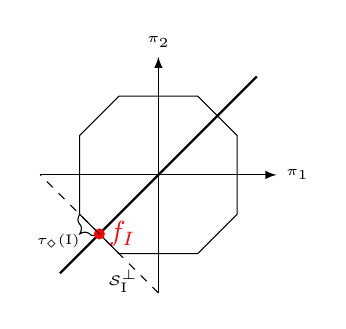
\begin{tikzpicture}[decoration={brace, amplitude=5pt}]
        % \filldraw[fill=black!5,dotted] (-1,-0.5) -- (-0.5,-1) -- (1,0.5) -- (0.5,1) -- cycle;
        \draw[-latex] (-1.5,0) -- (1.5,0) node[right] {\tiny $\pi_1$};
        \draw[-latex] (0,-1.5) -- (0,1.5) node[above] {\tiny $\pi_2$};
        \draw (1,-0.5) -- (1,0.5) -- (0.5,1) -- (-0.5,1) -- (-1,0.5) -- (-1,-0.5) -- (-0.5,-1) -- (0.5,-1) -- cycle;
        \draw[thick] (-1.25,-1.25) -- (1.25,1.25);% node[above right];% {\tiny $\polydr{\PP_{\I}\pi}{\I}=1$};
        \draw[decorate, decoration={brace,mirror, amplitude=5pt}]
             (-1,-0.5) -- (-0.75,-0.75)
             node[midway, anchor=north east] {\tiny $\tau_\diamond(\I)$};
    %         \draw[->] (0.9,0.9) -- (0.75,0.75);
        % \fill[red] (0.75,0.75) circle (2pt);
        \fill[red] (-0.75,-0.75) circle (2pt) node[right]{$f_I$};
        \draw[dashed] (0,-1.5) -- (-1.5,0) node[midway, xshift=3mm, yshift=-6mm] {\tiny $\SS_{\I}^\perp$};
            \end{tikzpicture}
            \caption{Consider a SLOPE norm with $w=(1,1/2)$ and a pattern $I=(-1,-1)$.
            The thick black line corresponds to $\mathcal{S}_\I = \R(1,1)^\top$.
            The red dot represents the face projection $f_\I$.}\label{fig:tau}
\end{figure}




\begin{remark}\label{rem:tau_does_not_exist}
Recall that in general we have $1=\polydr{f_\I}{\I} \leq \polyd{f_\I}$.
The threshold $\tau_\diamond(\I)$ is well-defined if and only if the set $\{t\geq0\colon \forall\,\pi^\bot\in\SS_{\I}^\bot\,\,\,\, \cnorm{D\pi^\bot}\leq t\implies \polyd{f_{\I}+\pi^\bot}\leq 1\}$ is non-empty. Clearly, this set is non-empty if and only if $t=0$ is an element of this set if and only if $\polyd{f_\I}= 1$. 
\end{remark}

\begin{lemma}\label{lem:tau}
Assume that $\polyd{f_\I}=1$. Then,
\[
\tau_\diamond(\I)=  \inf_{\pi^\bot\in\SS_\I^\bot\colon \polyd{f_\I+\pi^\bot}> 1}\cnorm{D\pi^\bot}.
\]
\end{lemma}


In general, it is possible that $\tau_\diamond(\I)=0$ for some active set $\I$ and the following result characterizes this condition. This happens exactly when $f_\I$ belongs to the boundary of $\mathrm{ri}(F_\I)$. In Example \ref{ex:simple}, such a case occurs exactly if $\alpha\in\{-1,1\}$ or $\alpha^2+\beta^2=|\alpha|$.

\begin{lemma}\label{lem:tau_positive}
\[
\tau_\diamond(\I)>0 \quad\iff\quad f_\I\in\mathrm{ri}(F_\I).
\]
\end{lemma}

We note that the condition $f_\I\in\mathrm{ri}(F_\I)$ implies $\polyd{f_\I}=1$. 


\subsection{Second threshold}\label{sec:zeta}
The second threshold specifies a sufficient condition under which an element $x$ in the pattern subspace $\SS_y$ shares the same pattern as $y$, $\patt{x}=\patt{y}$. 
Concretely, it does so by imposing a bound on the distance between $x$ and $y$. 

In our setting---where $\R^m$ denotes the half-vectorization of symmetric matrices---we measure this distance using an arbitrary norm $\cnorm{\cdot}$ on $\R^{p^2}\supset\v{\mathrm{Sym}(p)}$. To streamline notation, we will write
$\patt{X}$ in place of $\patt{\vp{X}}$ for any $X\in\mathrm{Sym}(p)$. 

Let $\Mast$ denote the matrix-pattern subspace associated with the true concentration matrix $K^\ast$ (see Section \ref{sec:notation} for the formal definition) and $\Gamma^\ast = (K^\ast)^{-1}\otimes (K^\ast)^{-1}$.
\begin{defin}\label{def:zeta}
Define for $X\in\mathrm{Sym}(p)$, 
\begin{align*}
\zeta_\diamond(K^\ast) = 
\sup\{z>0 \colon \forall\,K \in\Mast,\quad \cnorm{\Gamma^\ast\v{K-K^\ast}} \le z \implies \patt{K}=\patt{K^\ast}\},
\end{align*}
where $\Gamma^\ast=\Sigma^\ast\otimes\Sigma^\ast$.
\end{defin}

We now show that this supremum can be characterized as the distance from $x$ to the complement of its pattern-equivalence class in $\SS_x$: 
\begin{lemma}\label{lem:zeta} We have
\begin{align*}
\zeta_\diamond(K^\ast) 
 = 
\inf_{\substack{K\in\Mast\\
      \patt{K}\neq\patt{K^\ast}}} \cnorm{\Gamma^\ast\v{K-K^\ast}}.
\end{align*}
Moreover, if $\cnorm{\cdot}=\|\cdot\|_\infty$,  $x^\ast=\vp{K^\ast}$ and $\SS^\ast=\SS_{x^\ast}$, then 
\begin{align*}
\zeta_\diamond(K^\ast) 
 \geq  \opnorm{K^\ast}_\infty^{-2}\!\!\!\inf_{\substack{x\in\SS^\ast\\
      \patt{x}\neq\patt{x^\ast}}} \!\!\! \|x-x^\ast\|_\infty.
\end{align*}
\end{lemma}






\section{Main results}\label{sec:main}

\subsection{Setting and notation}\label{sec:notation}

We introduce a polyhedral gauge $\norm$ on $\mathrm{Sym}(p)$, defined as
\[
\norm(X) = 2 \poly{ \vp{X}},
\]
where $\poly{\cdot}$ is an atomic norm on $\R^m=\vp{\mathrm{Sym}(p)}$, $m=p(p-1)/2$.  

The dual gauge associated with $\norm$ on $\mathrm{Sym}_0(p)$ is given by 
\begin{align*}
	\normd(Y) &= \sup_{\substack{X\in \mathrm{Sym}_0(p) \\ \norm(X)\leq 1}}  \tr{Y X}   = \polyd{\vp{Y}},\qquad Y\in\mathrm{Sym}_0(p). 
\end{align*}

Let $\Sigma^\ast\in\mathrm{Sym}_+(p)$ and $K^\ast=(\Sigma^\ast)^{-1}$ be the true covariance and precision matrices, respectively. 
Let $\Sast = \SS_{\vp{K^\ast}}$ be the pattern subspace of the true concentration matrix and let $\I^\ast$ denote the corresponding active set so that $\Sast=\SS_{\I^\ast}$.  We also define the matrix pattern subspace of  $\mathrm{Sym}(p)$  by
\[
\Mast = \{ K\in\mathrm{Sym}(p)\colon \vp{K} \in \Sast\}.
\]


Define the $p^2\times p^2$ matrix 
\[
\Gamma^\ast=\Sigma^\ast\otimes\Sigma^\ast
\]
and its block components 
\[
\Gamma^\ast_{1,1} =  \PM \Gamma^\ast \PM\quad\mbox{and}\quad\Gamma^\ast_{2,1} =  (I_{p^2}-\PM) \Gamma^\ast \PM,
\]
where $\PM\in\mathrm{Sym}(p^2)$ is the orthogonal projection matrix from $\v{\mathrm{Sym}(p)}$ onto $\v{\Mast}$. 

We denote $(\Gamma^\ast_{1,1})^+$ as the Moore-Penrose inverse of $\Gamma^\ast_{1,1}$ and define the matrix
\[
\Q=\Gamma^\ast(\Gamma_{1,1}^\ast)^{+}.
\]
Applying properties of the Moore-Penrose inverse yields
\[
\Q - \PM = \Gamma_{2,1}^\ast (\Gamma_{1,1}^\ast)^{+}.
\]

Let $\cnorm{\cdot}$ be an arbitrary norm (an actual norm)
on $\R^{p^2}$ and let  $\copnorm{\cdot}$ denote the operator norm induced by $\cnorm{\cdot}$. 

\begin{defin}[Irrepresentability condition]
There exists $\alpha\in(0,1)$ such that 
\begin{align}\label{eq:irrep0}
	\cnorm{ \Gamma_{2,1}^\ast (\Gamma_{1,1}^\ast)^{+}D f_{\I^\ast}}\leq (1-\alpha)\tau_\diamond(\I^\ast), 
\end{align}
where $f_{\I^\ast}$ is the face projection of $F_{\I^\ast}$ and $D$ is the duplication matrix.
\end{defin}


\begin{defin}\label{def:c}
	Let $c_\diamond$ be a constant for which
		\[
	\cnorm{D \pi} \leq c_\diamond \polydr{\pi}{\I^\ast},\quad\forall \, \pi\in\Sast.
	\]
	Additionally, let $\cH$ be a constant for which 
	\[
	\copnorm{\Sigma^\ast\Delta\otimes I_p} \leq \cH \cnorm{\Gamma^\ast\v{\Delta}},\quad\forall\, \Delta\in \Mast.
	\]
\end{defin}
In Lemma \ref{lem:kappainfty} we show that if $\cnorm{\cdot}$ is the $\ell_\infty$-norm, then one can take $\cH = \|\v{K^\ast}\|_1=\sum_{i,j}|K^\ast_{i,j}|$. 



\subsection{Main Theorems}\label{subsec:main}
We consider the following optimization problem:
\begin{align}\label{eq:hatK}
	\hat K = \argmin_{K\in \mathrm{Sym}_+(p)} \left\{ \tr{\hat{\Sigma}K}-\log\det(K)+\lambda \norm(K)\right\}.
\end{align}

Although we do not explicitly assume $f_{\I^\ast}\in\mathrm{ri}(F_{\I^\ast})$, the following result requires that $\tau_\diamond(\I^\ast)>0$, which through Lemma \ref{lem:tau_positive} implies that $f_{\I^\ast}\in\mathrm{ri}(F_{\I^\ast})$.  This result is supplemented with the study of the case when $\tau_\diamond$ does not exists, see Appendix \ref{app:pr}. 

The thresholds $\tau$ and $\zeta$ are defined in Definitions \ref{def:tau} and \ref{def:zeta}, respectively.

\begin{thm}\label{thm:patt_recov}
	Assume that there exists $\alpha\in(0,1)$ such that \eqref{eq:irrep0} holds. 
	Suppose that for some $(r,\lambda)\in(0,1)\times (0,\infty)$, we have $r\leq \cH\zeta_\diamond(K^\ast)$ and
	\begin{align}\label{eq:smallr}
		\cnorm{\v{\hat{\Sigma}-\Sigma^\ast}}\leq \min\left\{\frac{r}{\cH\copnorm{\Q}} - \lambda\,c_\diamond, \frac{\alpha\,\lambda\,\tau_\diamond(\I^\ast)}{\copnorm{I_{p^2}-\Q}}
		\right\} - \frac1{\cH}\frac{r^2}{1-r}.
	\end{align}
	Let $\hat{K}$ be the unique solution to \eqref{eq:hatK}. Then,  $\patt{\hat{K}}=\patt{K^\ast}$ and 
	\[
	\cnorm{\Gamma^\ast\v{\hat{K} - K^\ast}}\leq \frac{r}{\cH}.
	\]
\end{thm}


Below we present the optimized (i.e. for $r$ and $\lambda$ for which $\delta$ is as large as possible) version of Theorem \ref{thm:patt_recov}.
\begin{thm}\label{cor:main} 
Assume that $\tau_{\diamond}>0$ and that there exists $\alpha>0$ such that \eqref{eq:irrep0} holds. 

Define  
\[
M = \frac{ \alpha\tau_\diamond}{\copnorm{\Q}( \copnorm{I_{p^2}-\Q} c_\diamond+\alpha\tau_\diamond)}\quad\mbox{and}\quad r = \min\left\{ 1- \frac{1}{\sqrt{1+M}},\cH\,\zeta_\diamond\right\}
\]
and
\[
     \delta = \begin{cases}
       \frac{\left(\sqrt{1+M}-1\right)^2}{\cH}, & \mbox{if }r \leq \cH \zeta_\diamond
       \\ M \zeta_\diamond-\frac{\cH\zeta_\diamond^2}{1-\cH\,\zeta_\diamond}, & \mbox{if }r > \cH\,\zeta_\diamond.\end{cases}
\]
Let $\hat{K}$ be the unique solution to \eqref{eq:hatK} with
\[
\lambda=\frac{r \copnorm{I_{p^2}-\Q}}{\cH\copnorm{\Q}(  c_\diamond \copnorm{I_{p^2}-\Q}+\alpha\tau_\diamond)}
\]
If 
\[
\cnorm{\v{\hat{\Sigma}-\Sigma^\ast} }< \delta
\]
then $\patt{\hat{K}}=\patt{K^\ast}$ and
\[
\cnorm{\Gamma^\ast\v{\hat{K}-K^\ast}}\leq \frac{1}{\cH}\left(1-\frac{1}{\sqrt{1+M}}\right). 
\]
\end{thm}

We note that $\delta$ defined in Theorem \ref{cor:main} is always positive. Moreover, one has the following asymptotic expansions:
    \begin{align*}
\left(\sqrt{1+M}-1\right)^2  =\frac{M^2}{4} + O(M^3)\quad\mbox{and}\quad
1-\frac{1}{\sqrt{1+M}} = \frac{M}{2} + O(M^2). 
\end{align*}

We consider three natural choices for the norm $\cnorm{\cdot}$ on $\R^{p^2}$. 
\begin{itemize}
	\item  Norm based on a dual norm: for $X\in\mathrm{Mat}(p\times p)$, define
	\[
	\cnorm{\v{X}} =\max\left\{\polyd{\vp{X}}, \polyd{\vp{X^\top}}, \|(X_{i,i})_{i=1}^p\|_\infty\right\}.
	\]
	This choice aligns the measure $\tau_\diamond$ of the perturbation $\pi^\bot$	using the same norm that defines the feasible region. 
Consequently, $\tau_\diamond$ becomes intrinsically linked to the geometry of the dual ball $B^\ast$ and becomes a dimensionless quantity.
	\item $\ell_\infty$-norm: for the specific case of GLASSO, the operator norm defined above coincides with the $\ell_\infty$-norm. This makes the $\ell_\infty$-norm a particularly natural choice, as adopted by \cite{ravikumar2011graphical}. To facilitate a direct comparison with GLASSO results when considering other atomic norms, using the $\ell_\infty$ is often the most convenient approach.
	\item  	The Mahalanobis norm: a weighted $\ell_2$ norm as defined in Appendix \ref{app:Maha}. For this specific norm, we have $\copnorm{\Q}=\copnorm{I_{p^2}-\Q}=\cH=1$, which greatly simplifies formulations of our results. However, this norm is generally not compatible with the irrepresentability condition. When formulated using the Mahalanobis norm, condition \eqref{eq:irrep0} tends to be much more restrictive than when expressed using the other two norms.
\end{itemize}



\subsection{Finite sample theory and concentration results}\label{sec:FST}

Theorems \ref{thm:patt_recov} and \ref{cor:main} establish conditions for pattern recovery that depend on a bound of the form
\[
\cnorm{\v{\hat{\Sigma}-\Sigma^\ast}} < \delta,
\]
where $\hat\Sigma = \hat{\Sigma}_n= \frac{1}{n} \sum_{i=1}^n X^{(i)} (X^{(i)})^\top$ is the sample covariance matrix based on $n$ i.i.d. observations of vector $X$. Since $\delta$ is independent of $n$, this condition can be satisfied with arbitrarily high probability by choosing a sufficiently large sample size. That is, for any $q\in(0,1)$, there exists a threshold $n_0$ such that for all $n\geq n_0$, 
\[
\P( \cnorm{ \v{\hat{\Sigma}_n-\Sigma^\ast}}\leq \delta)\geq q. 
\]
The specific value of $n_0$ and its asymptotic scaling heavily depends on the data distribution, particularly the tail behavior of $X$.   For instance, a distinction is often made between sub-Gaussian distributions and those with heavier, polynomial-type tails, each leading to different concentration rates.  

When $\cnorm{\cdot}$ is the $\ell_\infty$-norm then the relevant concentration inequalities can be found in \cite[Section 2.3 and Lemma 8]{ravikumar2011graphical}. Concentration results for the spectral norm are particularly well-established in the literature, see  \cite{CON5},  \cite{CON1}, \cite[Section 5.4.3]{CON3},  \cite{CON4}.





\subsection{GLASSO and relation to previous results}\label{sec:glasso}



Our general result builds upon and extends foundational results, particularly Theorems 1 and 2 from \cite{ravikumar2011graphical}. To make the comparison with \cite{ravikumar2011graphical} more meaningful, we assume a stronger version of irrepresentability condition, see \eqref{eq:irrepglasso} below. 
Recall that the $\ell_\infty$ operator norm $\opnorm{\cdot}_\infty$ is the maximum absolute row sum of the matrix.

Let $S = \{ (i,j)\colon K^\ast_{i,j}\neq 0\}$ be the support of the true precision matrix $K^\ast$, and write $S^c$ for its complement. Define $d$ as the largest number of non-zero entries in any row of $K^\ast$, and set $\Theta_{\min} = \min_{(i,j)\in S} |K_{i,j}^\ast|$. Finally, denote by $\Gamma_{S,S}^\ast$ (resp. $\Gamma_{S^c,S}^\ast$) the submatrix of $\Gamma^\ast$ obtained by selecting the rows in $S$ (resp. $S^c$) and the columns in $S$.


\begin{thm}[$\ell_1$-norm]\label{thm:glasso} 
	Assume that 
	\begin{align}\label{eq:irrepglasso}
	\opnorm{\Gamma_{S^c,S}^\ast(\Gamma_{S,S}^\ast)^{-1}}_\infty\leq 1-\alpha.
	\end{align}
	Let $\hat{K}$ be the unique solution to \eqref{eq:hatK} with 
	\[
	\lambda=\frac{ \min\left\{ \tfrac{\alpha}{4}, \cH \opnorm{K^\ast}_\infty^{-2} \Theta_{\min}\right\}(1-\alpha/2)}{\cH}
	\] 
    and define 
\[
 \delta=\begin{cases}
 \frac{\alpha^2}{16\,\cH}\left(1-\frac{\alpha}{3}\right), & \mbox{if }\alpha \leq 4 \cH\opnorm{K^\ast}_\infty^{-2} \Theta_{\min},\\
\frac{\alpha}{6} \opnorm{K^\ast}_\infty^{-2} \Theta_{\min}, & \mbox{otherwise},
        \end{cases}
        \]
where $\cH = \min\{ d \opnorm{\Sigma^\ast}_\infty \opnorm{K^\ast}_\infty^2, \|\v{K^\ast}\|_1\}$. 
If
	\[
	\|\v{\hat{\Sigma}-\Sigma^\ast} \|_\infty\leq  \delta,
	\]
	then $\mathrm{sign}(\hat{K})=\mathrm{sign}(K^\ast)$ and 
\[
	\|\v{\hat{K}-K^\ast}\|_\infty \leq \frac{\alpha \opnorm{K^\ast}_\infty^2}{4\,\cH} = \frac{\alpha}{4}\max\left\{
    \frac{1}{d \opnorm{\Sigma^\ast}_\infty}, \frac{\opnorm{K^\ast}^2_\infty}{\|\v{K^\ast}\|_1}
    \right\}.
		\]
\end{thm}

For a clear comparison with our findings, we first restate key results of \cite{ravikumar2011graphical} in an equivalent form. In doing so, we also identify and propose a correction for an issue in the formulation and proof of their Theorems 1/2. This correction is related to a small error in the proof of their Theorem 1, which unfortunately results in an incorrect statement. 

Recall that $\Gamma^\ast=\Sigma^\ast\otimes \Sigma^\ast$ and  define the quantities
\begin{align*}
	\kappa_{\Sigma^\ast}=\opnorm{ \Sigma^\ast}_{\infty},\quad
	\kappa_{\Gamma^\ast}=\opnorm{ (\Gamma^\ast_{S,S})^{-1}}_{\infty}.
\end{align*} 

\textbf{Theorems 1 and 2  in \cite{ravikumar2011graphical}, restated.}
\textit{
	Assume \eqref{eq:irrepglasso} and define 
		\begin{align}\label{eq:29}
\delta_R = 	\left( 6 \left(1+\frac8\alpha\right)d \,\kappa_{\Sigma^\ast} \kappa_{\Gamma^\ast} \max\{1, \kappa_{\Sigma^\ast}^2 \kappa_{\Gamma^\ast}\}\right)^{-1}.
	\end{align}
	Let $\hat{K}$ be the unique GLASSO estimator with tuning parameter $\lambda = (8/\alpha)\delta_R$. If
\[
		\| \v{\hat{\Sigma}_n-\Sigma^\ast}\|_\infty \leq \delta_R,
\]
then the following hold:
\begin{itemize}
	\item element-wise $\ell_\infty$-bound: 
		\[
	\|\v{\hat{K}-K^\ast}\|_\infty \leq 2\left(1+\frac{8}{\alpha}\right)\kappa_{\Gamma^\ast}\delta_R.
	\]
	\item pattern recovery guarantees: if $K^\ast_{i,j}=0$, then $\hat{K}_{i,j}=0$. If additionally 
	\begin{align}\label{eq:trueedges}
		\Theta_{\min}>2\left(1+\frac{8}{\alpha}\right)\kappa_{\Gamma^\ast}\delta_R.
	\end{align}
	then $\mathrm{sign}(\hat{K})=\mathrm{sign}(K^\ast)$.
\end{itemize}
}
This formulation connects to the original probabilistic statement in \cite{ravikumar2011graphical} by noting that for any $\tau > 2$, there exists a sample size $n_0$ (since $\delta$ is independent of $n$) such that for $n \ge n_0$, the condition $\| \v{\hat{\Sigma}_n-\Sigma^\ast}\|_\infty\leq \delta_R$ holds with probability at least $1-1/p^{\tau-2}$. If all true non-zero edges satisfy \eqref{eq:trueedges}, then full strong pattern recovery is achieved, which gives  essentially their Theorem 2.


The derivation of $\delta$ in \cite{ravikumar2011graphical} involves several lemmas. Our work modifies and generalizes these to our atomic norm framework. However, we first address an issue within their original argument for the $\ell_1$-norm.

First we note that the term $\max\{1, \kappa_{\Sigma^\ast}^2 \kappa_{\Gamma^\ast}\}$ in \eqref{eq:29} simplifies to $\kappa_{\Sigma^\ast}^2 \kappa_{\Gamma^\ast}$. This is because 
\[
\kappa_{\Sigma^\ast}^2 \kappa_{\Gamma^\ast} = \opnorm{\Sigma^\ast}_\infty^2 \opnorm{(\Gamma_{S,S}^\ast)^{-1}}_\infty \geq \opnorm{ \Gamma^\ast (\PP_S\Gamma^\ast\PP_S)^{+}}_\infty,
\]
where $\PP_S$ is the orthogonal projection matrix onto the vectorized model subspace, cf. definition of $\Q$ in Section \ref{sec:notation}. Since $\mathrm{Q}= \Gamma^\ast (\PP_S\Gamma^\ast\PP_S)^{+}$ is a projection matrix, its operator norm is at least $1$. 
Thus, \eqref{eq:29} can be rewritten as
\begin{align}\label{eq:ravierror}
	\delta_R = \left( 6 \kappa_{\Sigma^\ast}^3 \kappa_{\Gamma^\ast}^2 d\left(1+\frac8\alpha\right)\right)^{-1}.
\end{align}
With $\lambda = 8\delta_R/\alpha$, the authors of \cite[line 11, page 963]{ravikumar2011graphical}) state
\[
\|\v{R(\Delta)}\|_{\infty} \leq \left\{6 \kappa_{\Sigma^\ast}^3 \kappa_{\Gamma^\ast}^2 d\left(1+\frac8\alpha\right)^2\delta_R \right\}\frac{\alpha \lambda}{8}.
\]
Their objective is to show $\|\v{R(\Delta)}\|_{\infty}\leq (\alpha \lambda)/8$ and then to apply their Lemma 5. However, substituting \eqref{eq:ravierror} into the above inequality only yields
\[
\|\v{R(\Delta)}\|_{\infty}\leq \left(1+\frac8\alpha\right) \frac{\alpha \lambda}{8}.
\]
Since $\alpha$ is typically small, the term $(1+8/\alpha)$ can be significant. This means the condition $\|\v{R(\Delta)}\|_{\infty}\leq (\alpha \lambda)/8$ is not met by their argument under  \eqref{eq:ravierror}. This invalidates the subsequent application of their Lemma 5 and leaves the proof of Theorem 1 incomplete as stated.

To rectify the proof, a different definition of $\delta_R$ is required. Specifically, to ensure $\|\v{R(\Delta)}\|_{\infty}\leq (\alpha \lambda)/8$, one may take 
\begin{align}\label{eq:goodDelta}
\delta_R = \left( 6 \kappa_{\Sigma^\ast}^3 \kappa_{\Gamma^\ast}^2 d\left(1+\frac8\alpha\right)^2\right)^{-1}.
\end{align}
This corrected definition includes an additional factor of $(1+8/\alpha)$ in the denominator compared to \eqref{eq:29} and \eqref{eq:ravierror}.

It is worth noting that this discrepancy may affect the results of subsequent works that directly rely on the precise formulation of \cite[Theorem 1]{ravikumar2011graphical}, for instance, in \cite[Proposition 11.10]{Wainwright_2019}, where one should have $n> c_0(1+8 \alpha^{-1})^4m^2\log d$ rather than $n> c_0(1+8 \alpha^{-1})^2m^2\log d$. Interestingly, \cite{FUN_GLASSO}, which extends the approach of \cite{ravikumar2011graphical} to functional graphical LASSO, appears to use a condition consistent with our corrected bound (cf. (6.2) in their Theorem 5), though they do not explicitly report the error in the original paper.

Now we are ready to make a comparison, see also Section \ref{sec:num} for numerical experiments. For simplicity, we will only compare the terms not related to $\Theta_{\min}$. Thus, by Theorem \ref{thm:glasso}, we have 
\[
\delta \approx \frac{ \alpha^2}{16\min\{d \,\kappa_{\Sigma^\ast} \opnorm{K^\ast}^2 _\infty, \|\v{K^\ast}\|_1 \}},
\]
while the leading term of \eqref{eq:goodDelta} is 
\[
\delta_R\approx  \frac{1}{384} \frac{\alpha^2 }{d\,\kappa_{\Sigma^\ast}^3 \kappa_{\Gamma^\ast}^2} \approx \delta \cdot  \frac{1}{24} \min\left\{ \left(
\frac{  \opnorm{K^\ast}_\infty}{ \kappa_{\Sigma^\ast} \kappa_{\Gamma^\ast}}\right)^2 ,\frac{ \|\v{K^\ast}\|_1 }{ d\,\kappa_{\Sigma^\ast}^3 \kappa_{\Gamma^\ast}^2} 
\right\}
\]
Larger values of $\delta$ lead to stronger pattern-recovery guarantees. While our bound already improves on the numerical constant reported by \cite{ravikumar2011graphical}, the more consequential advantage is the superior asymptotic behavior of the  term 
\[
\min\left\{ \left(
\frac{  \opnorm{K^\ast}_\infty}{ \kappa_{\Sigma^\ast} \kappa_{\Gamma^\ast}}\right)^2 ,\frac{ \|\v{K^\ast}\|_1 }{ d\,\kappa_{\Sigma^\ast}^3 \kappa_{\Gamma^\ast}^2} 
\right\}. 
\]
This term is upper bounded by $\opnorm{\Sigma^\ast}_\infty \opnorm{K^\ast}_\infty$, but in our numerical examples from Section \ref{sec:num} it is always less than $1$. Below, we also consider explicit example for which this term is of order $1/p^3$, so that our $\delta$ is asymptotically $p^3$ larger than $\delta_R$. 
\begin{example}
Let $\rho\in(-1/(p-2),1)$ and 
\[
K_{ij}^\ast = \begin{cases}
	1, & \mbox{if }i=j,\\
	\rho, & \mbox{if }i\neq j\mbox{ and } \max\{i,j\}<p,\\
	0, & \mbox{if }i\neq j\mbox{ and } \max\{i,j\}=p.
\end{cases}
\]
Then $d=p-1$ and direct calculation shows that 
\begin{gather*}
	\kappa_{\Gamma^\ast} = (1+(p-2)\rho)^2, \qquad 	\opnorm{K^\ast}_\infty = 1+(p-2)|\rho|,\\
	\kappa_{\Sigma^\ast}  =  \frac{1-\rho+(p-2)(\rho+|\rho|)}{(1-\rho)(1+(p-2)\rho)},\qquad \|\v{K^\ast}\|_1 = p+|\rho|(p-1)(p-2).
\end{gather*}
Thus, for any $\rho\in(0,1)$ (case $\rho=0$ is trivial, while $\rho<0$ is asymptotically forbidden), we obtain as $p\to\infty$, 
\[
\min\left\{ \left(
\frac{  \opnorm{K^\ast}_\infty}{ \kappa_{\Sigma^\ast} \kappa_{\Gamma^\ast}}\right)^2 ,\frac{ \|\v{K^\ast}\|_1 }{ d\,\kappa_{\Sigma^\ast}^3 \kappa_{\Gamma^\ast}^2} 
\right\}\sim \left(\frac{1-\rho}{2\rho}\right)^3\frac{1}{p^3}
\]
(the first term is of order $p^{-2}$), which eventually implies that for positive $\rho$ and large $p$, we have
\[
\delta_R \approx  \left(\frac{1-\rho}{\rho}\right)^3\frac{\delta}{192\, p^3}. 
\]
\end{example}




\section{Numerical experiments}\label{sec:num}

Consider a simple undirected graph $G=(V,E)$ with $V=\{1,\dots,p\}$. Denote by $A_G$ its adjacency matrix. We represent the edge set $E$ as a subset of  ordered pairs $(i,j)\in V\times V$, $i>j$.  Throughout this section we set, for $i\neq j$, 
$K^\ast_{ij} = \rho\neq0$ if $\{i,j\}\in E$ and $K^\ast_{ij}=0$ otherwise.  Thus, we have 
\[
x^\ast: =\vp{K^\ast}=\rho \,\vp{A_G}\in\R^m,
\]
where $\rho\neq0$ and $m=p(p-1)/2$.  We enumerate entries of $\vp{K^\ast}$ via ordered pairs $e=(i,j)$, $i>j$. Thus, $x^\ast_{e} = \rho$ if and only if $e\in E$. 
Let $d:=\max_{i\in V}\deg_G(i)+1$ denote one plus the maximum vertex degree.

We investigate three regularizers $\poly{\cdot}$: the $\ell_1$ norm, the $\ell_{\infty}$ norm, and the SLOPE norm $\|\cdot\|_w$ with weight vector $w$ (see Example \ref{ex:SLOPE}). 
We consider $\cnorm{\cdot}=\|\cdot\|_\infty$. 
To ease the notation, we will use the norm subscripts $1$, $\infty$ and $w$ to indicate objects corresponding to a given norm.

The $\ell_1$-pattern $\mathrm{patt}_1$ can be identified with the $\mathrm{sign}$ function, while the $\ell_\infty$-pattern corresponds to the signs of the entries that attain the maximum absolute value, see Examples \ref{ex:l1} and \ref{ex:linfty}. The SLOPE pattern of $x\in\R^m$ can be uniquely represented by the vector $M_x\in\R^m$ defined by 
\[
(M_x)_i = \mathrm{sign}(x_i )\mathrm{rank}(|x|)_i,\quad i=1,\ldots,m,
\]
see \cite[Definition 2.1]{7aut}.


 The corresponding pattern subspaces for $x^{\ast}$ are
\[
\begin{array}{@{}l@{\quad}l@{}}
  \begin{aligned}
    \SS_1 &= \{\,x\in \R^m\colon x_e=0 \text{ for } e\notin E\},\\
    \SS_\infty &= \{\,x\in \R^m\colon x_e = x_{e'} \text{ for all }e,e'\in E\},
  \end{aligned}
  &
  \vcenter{\hbox{\qquad $\displaystyle \SS_w \;=\;\SS_1\cap \SS_\infty$.}}
\end{array}
\]


Denote $k = |E|/2$. The face projections are 
\begin{align*}
f_1 = \mathrm{sign}(x^\ast) = \mathrm{sign}(\rho)\vp{A_G},\qquad f_\infty = f_1 / \|f_1\|_1, \qquad  f_{w}=w_{(1,k)} f_1, 
\end{align*}
where $w_{(i,j)}$ denotes the average $\frac{1}{j-i+1} \sum_{\ell=i}^j w_\ell$. Note that $\|f_1\|_1 =k$. 
Moreover, 
\[
\tau_1=1,\quad \tau_\infty = k^{-1}, \quad 
\tau_w = \min\left\{ h(w_1,\ldots,w_k), w_{(k+1,m)}\right\},
\]
with $h$ is defined in Lemma~\ref{lem:SLOPEtuning}, and 
\[
c_1 = 1, \qquad c_\infty = 1,\qquad c_w =  1/w_{(1,k)}
\]
and (cf. the proof of Theorem \ref{thm:glasso} and Lemma \ref{lem:kappainfty})
\[
\cH_1=\cH_w=\min\{ d\, \opnorm{\Sigma^\ast}_\infty \opnorm{K^\ast}_\infty ^2, \|\v{K^\ast}\|_1\}  \qquad \cH_\infty =\|\v{K^\ast}\|_1. 
\]
By the second part of Lemma \ref{lem:zeta}, we have
\begin{align*}
\zeta_\diamond(K^\ast) 
\geq \opnorm{K^\ast}_\infty^{-2}\!\!\!\inf_{\substack{x\in\SS^\ast\\
      \patt{x}\neq\patt{x^\ast}}} \!\!\! \|x-x^\ast\|_\infty.
\end{align*}
If $x\in \SS_1$ and $\mathrm{patt}_1(x)\neq\mathrm{patt}_1(x^\ast)$, then there exists $e\in E$ such that $\mathrm{sign}(x_e)\neq \mathrm{sign}(x_e^\ast)=\mathrm{sign}(\rho)$. If $x\in \SS_\infty$ and $\mathrm{patt}_\infty(x)\neq\mathrm{patt}_\infty(x^\ast)$, then there exists $e\notin E$ such that $|x_e|\geq |\rho|$ or there exists $e\in E$ with $\mathrm{sign}(x_e)\neq \mathrm{sign}(\rho)$.
If $x\in \SS_w$ and $\mathrm{patt}_w(x)\neq\mathrm{patt}_w(x^\ast)$, then $x = \gamma\, x^\ast$ for some $\gamma\leq 0$. In each case, we obtain the lower bound of the form
\begin{align*}
\zeta_\diamond(K^\ast) &\geq  \opnorm{K^\ast}^{-2}_\infty |\rho|.
\end{align*}


We consider four graph families $G=(\{1,\ldots,p\},E)$:
\begin{itemize}
	\item Chain: $\Sigma^{\ast}_{ii}=1$, $\Sigma^{\ast}_{ij} = 0.2$ for $\{i,j\}\in E$ and $K^\ast_{ij}=0$ for $\{i,j\}\notin E$; here $\rho=-5/24$,
	\item Hub (star): $\Sigma^\ast_{ii}=1$, $\Sigma^{\ast}_{ij} = 2.5/(p-1)$ for $\{i,j\}\in E$ and  $K^\ast_{ij}=0$ for $\{i,j\}\notin E$; here $\rho=-2.5(p-1)/((p-1)^2-2.5^2)$,
	\item Four-nearest neighbor grid: $K_{ii}^\ast=1$ and $K^\ast_{1j}=0.1=\rho$ for $\{i,j\}\in E$ and $K^\ast_{ij} = 0$ otherwise,
	\item Dense: $K^\ast_{ii}=1$, $K^\ast_{ij}=0.1=\rho$ if $\max\{i,j\}<p$ and $i\neq j$  and $K^\ast_{ij}=0$  otherwise. 
\end{itemize}




\subsection{Irrepresentability condition}
In view of $\cnorm{\cdot}=\|\cdot\|_\infty$, the irrepresentability condition \eqref{eq:irrep0} becomes (respectively for $\poly{\cdot}=\|\cdot\|_1, \|\cdot\|_\infty, \|\cdot\|_w$)
\begin{gather*}
	\| (I_{p^2}-\PP_1) \Gamma^\ast  (\PP_1\Gamma^\ast \PP_1)^+ f_1\|_\infty \leq (1-\alpha), \\
	\| (I_{p^2}-\PP_\infty) \Gamma^\ast  (\PP_\infty \Gamma^\ast \PP_\infty)^+  f_1 \|_\infty \leq (1-\alpha),\\
	\| (I_{p^2}-\PP_1 \PP_\infty) \Gamma^\ast  (\PP_\infty\PP_1 \Gamma^\ast \PP_1\PP_\infty)^+  f_1 \|_\infty \leq  (1-\alpha) \frac{\tau_w}{w_{(1,k)}},
\end{gather*}
where $\PP_1$ and $\PP_\infty$ are the orthogonal projections onto $\mathcal{M}_1 $ and $\mathcal{M}_\infty$, respectively. 

The term on the left-hand side of the third inequality is independent of the weight sequence $w$.  For the OSCAR weights (linearly decreasing from $1$ to $1/(2m-1)$; \citealp{OSCAR08}) one finds, using Appendix~\ref{app:slope} and Lemma~\ref{lem:D1},
$\tau_w/w_{(1,k)} = (1/(2m-1))/((2m-1)/m)= 2/(p(p-1))$, which is very stringent. However, we may maximize  the right hand side so that the irrepresentability condition is less restrictive. E.g. adopting instead the tuned weights (see Lemma \ref{lem:SLOPEtuning})
\begin{align}\label{eq:specialSLOPE}
w_i = \begin{cases}
    1, & i \leq \lfloor k/2\rfloor,\\
    2/3, & i = \lceil k/2\rceil \mbox{ and }k\mbox{ is odd}, \\
    1/3, & i > \lceil\frac{k}{2}\rceil,
\end{cases}
\end{align}
leads to $
\tau_w/w_{(1,k)}=(1/3)/(2/3)=1/2$.

Table~\ref{tab:graph_comparison_simple} reports the left--hand sides above for $p\in\{16,64\}$ and the four graph topologies.  The attainable $\alpha$ values for the $\ell_{\infty}$ and SLOPE models are comparable with those for GLASSO.

\begin{table}[htbp]
	\centering
	\begin{tabular}{l cccccc} 
		\toprule
$\| (I_{p^2}-\PP) \Gamma^\ast  (\PP \Gamma^\ast \PP)^+  f_1 \|_\infty$		& \multicolumn{3}{c}{$p = 16$} & \multicolumn{3}{c}{$p = 64$} \\
		\cmidrule(lr){2-4} \cmidrule(lr){5-7} % Adjusted cmidrule to span 2 columns each
		Graph Type       & $1$ & $\infty$ & $w$ & $1$ & $\infty$ & $w$ \\
		\midrule
		Chain graph      & 4.0e-01 & 6.5e-02 & 4.0e-01 & 4.0e-01 & 7.3e-02 & 4.0e-01 \\
		Hub graph        & 3.3e-01 & 4.6e-13 & 3.3e-01 & 7.9e-02 & 1.7e-12 & 7.9e-02 \\
		Grid             & 4.0e-01 & 2.1e-02 & 4.2e-01 &  4.0e-01 & 2.9e-02 & 4.1e-01 \\
		Dense graph & 1.0e-15 & 1.1e-12 & 1.1e-12 & 2.4e-15 & 1.6e-09  &  1.6e-09  \\
		\bottomrule
	\end{tabular}
	\caption{Irrepresentability conditions for different graph types and $p$ values.}
	\label{tab:graph_comparison_simple}
\end{table}



\subsection{Comparison with Ravikumar et al. (2011)}

Table~\ref{tab:graph_comparison_simple2} contrasts  our bound $\delta$ from Theorem \ref{cor:main} (in the case $\poly{\cdot}=\|\cdot\|_1$ and $\cnorm{\cdot}=\|\cdot\|_{\infty}$) with the threshold $\delta_R$ from \citet{ravikumar2011graphical} (recall \eqref{eq:goodDelta}). Across all scenarios, our bound exceeds that of \citet{ravikumar2011graphical} by several orders of magnitude, yielding markedly stronger guarantees for pattern recovery.

\begin{table}[htbp]
	\centering
	\begin{tabular}{l cccc} 
		\toprule
		& \multicolumn{2}{c}{$p = 16$} & \multicolumn{2}{c}{$p = 64$} \\
		\cmidrule(lr){2-3} \cmidrule(lr){4-5} 
		Graph Type       & $\delta$ & $\delta_{R}$ & $\delta$ & $\delta_{R}$ \\
		\midrule
		Chain graph      & 1.9e-03 & 1.6e-05 & 1.9e-03 & 1.6e-05 \\
		Hub graph        & 1.1e-03 & 2.3e-08 & 6.3e-04 & 1.6e-08 \\
		Grid             & 1.2e-03 & 1.0e-05 & 1.2e-03 & 9.4e-06 \\
		Dense graph & 1.4e-03 & 8.2e-07 & 1.1e-04 & 1.4e-09 \\
		\bottomrule
	\end{tabular}
	\caption{Comparison of $\delta$ and $\delta_{R}$ for different graph types and dimensions.}
\label{tab:graph_comparison_simple2}
\end{table}

\subsection{\texorpdfstring{Tightness of the threshold $\delta$}{Tightness of delta}}

For each graph topology we draw an error matrix $\mathcal{E}\in\mathrm{Sym}(p)$ in a way that $|\mathcal E|\sim\mathrm{Unif}(0,8\delta)$ and set $\hat\Sigma = \Sigma^{\ast}+\mathcal E$.  Using the optimal tuning parameter $\lambda$ from Theorem~\ref{cor:main}, we compute the estimator $\hat K$ with the penalty $\poly{\cdot}\in\{\|\cdot\|_1, \|\cdot\|_\infty, \|\cdot\|_w\}$.  Repeating this experiment $N=1\,000$ times we record the pairs $(\|\v{\hat{\Sigma}_i-\Sigma^{\ast}}\|_{\infty},\;\|\v{\hat{K}_i-K^{\ast}}\|_{\infty})$ and display the results as scatter plots.  
 We compare the theoretical $\delta$ with the empirical threshold
\[
\hat{\delta} = \min\{ \|\v{\hat{\Sigma}_i-\Sigma^{\ast}}\|_{\infty}\colon \patt{\hat{K}_i}=\patt{K^\ast}\}.
\]

In the case of GLASSO, we find that $\hat{\delta}$ exceeds the theoretical bound $\delta$ from Theorem \ref{cor:main} by only a factor of about $2$, see Figure \ref{fig:glasso}.

\begin{figure}[htbp]
	\includegraphics[width=0.8\textwidth]{GLASSO25.png}
\caption{GLASSO: Scatter plot of \(\|\v{\hat{\Sigma}-\Sigma^{\ast}}\|_{\infty}\) (x-axis) versus 
\(\|\v{\hat{K}-K^{\ast}}\|_{\infty}\) (y-axis) for $p=25$.  
The gray dashed line marks the theoretical threshold \(\delta\); the orange dashed line shows its empirical threshold \(\hat{\delta}\).  
Points are colored blue when the true pattern (sign) is recovered and red otherwise.}\label{fig:glasso}
\end{figure}


We carried out an analogous evaluation for the SLOPE penalty, using the weights specified in \eqref{eq:specialSLOPE}, and display the outcomes in Figure \ref{fig:slope}. The observed thresholds exceed the theoretical bounds by roughly a factor of $20$ on both chain and grid graphs, about $7$ on the hub graph, and near $4$ on the dense graph. This marked gap likely stems from our assessing deviations in the $\ell_\infty$ norm, which may not be the appropriate metric in this context. 

\begin{figure}[htbp]
	\includegraphics[width=0.8\textwidth]{SLOPE25.png}
\caption{SLOPE: Scatter plot of \(\|\v{\hat{\Sigma}-\Sigma^{\ast}}\|_{\infty}\) (x-axis) versus 
\(\|\v{\hat{K}-K^{\ast}}\|_{\infty}\) (y-axis) for $p=25$.  
The gray dashed line marks the theoretical threshold \(\delta\); the orange dashed line shows its empirical threshold \(\hat{\delta}\).  
Points are colored blue when the true pattern is recovered and red otherwise.}\label{fig:slope}
\end{figure}

We also explored the performance under the $\ell_\infty$-penalty, but there our theoretical guarantees proved overly conservative compared to simulation results for all graph topologies. We suspect this discrepancy arises because $\cnorm{\cdot}=\|\cdot\|_1$ fails to reflect the effective dimension reduction in the $\mathcal{S}_\infty$ subspace, causing the constant $\eta_\infty$ to be excessively large.

Our experiments were run using the GSLOPE implementation kindly provided by Prof. Ma{\l}gorzata Bogdan (\cite{graphSLOPE}).


\section{Roadmap to the Proofs}\label{sec:ProofSkeleton}
\subsection{Primal-dual witness method}\label{sec:pdwm}
We consider the original and the restricted problem:
\begin{align}\label{eq:hatK2}
	\hat K &= \argmin_{K\in \mathrm{Sym}_+(p)} \left\{ \tr{\hat{\Sigma}K}-\log\det(K)+\lambda \norm(K)\right\},\\
	\tilde K &=\argmin_{K\in \Mast\cap \mathrm{Sym}_+(p)} \left\{ \tr{\hat{\Sigma}K}-\log\det(K)+\lambda \norm(K)\right\}. \label{eq:tildeK}
\end{align}
Recall that $\norm$ is an atomic norm on $\mathrm{Sym}_0(p)$
(see Section \ref{sec:vectorization} for the definition of $\mathrm{Sym}_0(\R)$).
We define the corresponding restricted dual norm on $\Mast_0= \Mast\cap \mathrm{Sym}_0(p)$. Let $\norms = \norm\big|_{\Mast}$ and 
\[
\normsd(Y) = \sup\{ \scalar{Y}{X}\colon X\in\Mast_0, \norms(X)\leq 1\},\quad Y\in \Mast_0.
\]
It follows that $\normsd(Y) = \polydr{\vp{Y}}{\I^\ast}$ with $\I^\ast =\I_{\vp{K^\ast}}$. 

Let $\proj\colon \mathrm{Sym}(p)\to \Mast$ denote the orthogonal projection onto $\Mast$.
Define also the orthogonal projection matrix $\PM \in\mathrm{Sym}(p^2)$ such that for all $X\in\mathrm{Sym}(p)$, the following holds: 
\begin{align*}
	\v{\proj(X)}=\PM \v{X}.
\end{align*}
Note that we have $\vp{\proj(X)}=\PP_{\I^\ast} \vp{X}$ (recall Section \ref{sec:pattern}).

\begin{lemma}\label{lem:1}
	Assume that $\hat{\Sigma}$ has positive diagonal entries.
	\begin{itemize}
		\item[(i)] The optimization problem \eqref{eq:hatK2} has a unique solution $\hat{K}\in\mathrm{Sym}_+(p)$, which is characterized by
		$\hat{K}^{-1}-\hat{\Sigma} = \lambda\hat{\Pi}$, 
		where $\hat{\Pi}\in \partial \norm(\hat{K})$.
		\item[(ii)] The constrained optimization problem \eqref{eq:tildeK} has a unique solution 
		$\tilde{K}\in \Mast\cap\mathrm{Sym}_+(p)$, which is  characterized by $\proj(\tilde{K}^{-1}-\hat{\Sigma}) = \lambda\tilde\Pi$,
		where $\tilde\Pi\in \partial \norms(\tilde{K})$.
	\end{itemize}
\end{lemma}

To establish that the original estimator $\hat{K}$ belongs to the true model subspace $\Mast$, it suffices to prove that $\hat{K}=\tilde{K}$. In Lemma \ref{lem:1}, we define
\[
\hat{\Pi} = \frac{1}{\lambda}(\hat{K}^{-1}-\hat{\Sigma})\quad\mbox{and}\quad \tilde{\Pi} = \frac{1}{\lambda}\PM(\tilde{K}^{-1}-\hat{\Sigma}). 
\]
Let additionally
\begin{align*}
	\Pi = \frac{1}{\lambda}(\tilde{K}^{-1}-\hat{\Sigma}).
\end{align*} 
The next result establishes a condition under which $\Pi=\hat{\Pi}$; this, in turn, implies that $\hat{K}=\tilde{K}$, thereby ensuring that $\hat{K}$ belongs to the true pattern subspace $\Mast$. 


\begin{lemma}\label{lem:hatKtildeK}
	We have $\normd(\Pi)\leq 1$ if and only if $\hat{K}=\tilde{K}$. 
\end{lemma}

\subsection{The basic bounds}\label{sec:bb}
Next, we find a sufficient condition under which we have $\normd(\Pi)\leq 1$. This condition will be formulated in terms of a projection $\Q$, recall its definition from Section \ref{sec:notation}.

For $\Delta\in \Mast$ such that $K^\ast+\Delta$ is invertible,  define the residual matrix
\[
R(\Delta) = (K^\ast+\Delta)^{-1}-\Sigma^\ast+\Sigma^\ast\Delta\Sigma^\ast. 
\]
We note that $R(\tilde{K}-K^\ast)$ is the difference of  $\nabla(-\log\det(\tilde K)) = \tilde K^{-1}$ from its first-order Taylor expansion around $K^\ast$. 

Recall the definition of $\tau_\diamond$ in Definition \ref{def:tau}. We obtain
\begin{lemma}\label{lem:Vbound}
	Assume that $\patt{\tilde{K}}=\patt{K^\ast}$.
	If there exists $\alpha\in (0,1)$ such that \eqref{eq:irrep0} holds
	and
	\[
	\cnorm{ \v{R(\tilde{K}-K^\ast)}}+\cnorm{\v{\hat{\Sigma}-\Sigma^\ast}}\leq \frac{\alpha\,\lambda\, \tau_\diamond(\I^\ast)}{\copnorm{I_{p^2}-\Q}},
	\]
	then $\normd(\Pi) \leq 1$.
\end{lemma}



While the term $\cnorm{\v{\hat{\Sigma}-\Sigma^\ast}}$,      
is stochastic and cannot be directly controlled, standard concentration inequalities ensure it can be made arbitrarily small with high probability by increasing the sample size $n$. The term $\cnorm{ \v{R(\tilde{K}-K^\ast)}}$ will be handled using the following result. 


\begin{lemma}[Control of the residual term]\label{lem:Rbound}
	If $\Delta\in\Mast$ satisfies 
    \[
	\cH\cnorm{\Gamma^\ast\v{\Delta}}\leq r <1,\qquad\mbox{then}\qquad 
		\cnorm{\v{R(\Delta)}} \leq  \frac{1}{\cH}\frac{r^2}{1-r}.
	\]
\end{lemma}

\subsection{Fixed-point argument}\label{sec:fpa}
To obtain control over the difference $\tilde{\Delta}=\tilde{K}-K^\ast$, we employ a similar approach as in \cite{ravikumar2011graphical}. 
In this section,
we define a continuous mapping $F$ that admits the unique fixed point
\[
\Gamma^\ast \v{\tilde{K}-K^\ast}. 
\]
Next, we will show that $F$ is a self-map on a particular convex set. Consequently, Brouwer's fixed point theorem guarantees that this fixed point lies within that convex set.

Define the function $F\colon  \{ \Gamma^\ast\v{\Delta}\colon \Delta\in\Mast, \,\opnorm{\Sigma^\ast\Delta}<1 \} \to \Gamma^\ast\v{\Mast}$ by
\[
F\left(\Gamma^\ast\,\v{\Delta}\right) = \Q\,\v{(K^\ast+\Delta)^{-1}-\tilde{K}^{-1}} + \Gamma^\ast\,\v{\Delta}.
\]

We have $K^\ast+\Delta=K^\ast(I_p+ \Sigma^\ast\Delta)$ and since $\opnorm{\Sigma^\ast\Delta}<1$, the matrix $(I_p+ \Sigma^\ast\Delta)$ is invertible. Hence, $K^\ast+\Delta$ remains positive definite, ensuring that $F$ is well-defined. Here, $\opnorm{\cdot}$ can be arbitrary operator norm. 

\begin{lemma}\label{lem:Ffixed}
	$\Gamma^\ast\v{\tilde{\Delta}}$ is a fixed point of $F$ if and only if $\tilde\Delta = \tilde{K} - K^\ast$.
\end{lemma}



\begin{lemma}[Control of the deviation $\tilde{\Delta}$]\label{lem:Deltabound}
	Assume that $r\in(0,1)$ and $\lambda>0$ satisfy
	\begin{align}\label{eq:rb}
		\cnorm{\v{\hat{\Sigma}-\Sigma^\ast}}\leq \frac{r}{\cH \copnorm{\Q}} - \lambda c_\diamond - \frac{1}{\cH}\frac{r^2}{1-r}.
	\end{align}
	Then, $F$ has a unique fixed point $\Gamma^\ast\v{\tilde{K}-K^\ast}$, $\tilde{K}-K^\ast\in\Mast$, which satisfies 
	\begin{align*}
		\cnorm{\Gamma^\ast\v{\tilde{K}-K^\ast}}\leq 	\frac{r}{\cH}.
	\end{align*}
	If additionally, $r \leq \cH \zeta_{\diamond}(K^\ast)$,
	then $\patt{\tilde{K}}=\patt{K^\ast}$. 
\end{lemma}

From Lemma \ref{lem:Deltabound}, we obtain the following immediate result
\begin{Corollary}\label{cor:bound}
	Assume that  
$x := \cH(\cnorm{\v{\hat{\Sigma}-\Sigma^\ast}}  + \lambda\,c_\diamond) \leq  \frac{0.1}{\copnorm{\Q}^2}$.
	Then, $r=\copnorm{\Q} x+ 2 \copnorm{\Q}^3 x^2$ satisfies \eqref{eq:rb} and 
	\[
	\cnorm{\Gamma^\ast\v{\tilde{K}-K^\ast}} \leq  \frac{r}{\cH}\leq 1.2\copnorm{\Q} (\cnorm{\v{\hat{\Sigma}-\Sigma^\ast}}  + \lambda\,c_\diamond).
	\]
	
\end{Corollary}





\subsection{Proofs of the main results}\label{sec:mr}
\begin{proof}[Proof of Theorem \ref{thm:patt_recov}]
	Observe that condition \eqref{eq:smallr} implies condition \eqref{eq:rb} from Lemma \ref{lem:Deltabound}.
	By Lemma \ref{lem:Deltabound}, $F$ has a fixed point $\Gamma^\ast\v{\tilde{\Delta}}\in\Gamma^\ast\v{\Mast}$ such that
	\[
	\cH\cnorm{\Gamma^\ast\v{\tilde{\Delta}}}\leq r,
	\]
	where $\tilde\Delta = \tilde{K}-K^\ast$. Since $r\leq \cH\,\zeta_\diamond(K^\ast)$, we have $\patt{\tilde{K}}=\patt{K^\ast}$. 
	
	
	By Lemma \ref{lem:Rbound}, the residual term $R=R(\tilde{\Delta})$ satisfies 
	\begin{align*}
		\cnorm{ \v{R}} &\leq \frac{1}{\cH}\frac{r^2}{1-r}. 
	\end{align*}
	Using condition \eqref{eq:smallr}, we obtain
	\begin{align*}
		\cnorm{\v{R}}+\cnorm{\v{\hat{\Sigma}-\Sigma^\ast}} \leq\frac{1}{\cH} \frac{r^2}{1-r} + \cnorm{\v{\hat{\Sigma}-\Sigma^\ast}} \leq\frac{ \alpha\,\lambda\,\tau_\diamond(\I^\ast)}{\copnorm{I_{p^2}-\Q}}.
	\end{align*}
	Applying Lemma \ref{lem:Vbound}, we conclude that $\normd(\Pi)\leq 1$. Then, by Lemma \ref{lem:hatKtildeK}, it follows that $\hat{K}=\tilde{K}$, which completes the proof.
\end{proof}

\begin{proof}[Proof of Theorem \ref{cor:main}]
	The proof follows from Theorem \ref{thm:patt_recov} and Lemma \ref{lem:optim} with $\tau' = \tau/\copnorm{I_{p^2}-\Q}$.
\end{proof}

The proof of Theorem \ref{thm:glasso} is relegated to the Appendix \ref{app:proofs}. 


\bibliographystyle{plainnat}
\bibliography{GLASSO-20221101}

%\printbibliography

\appendix 
%\setcounter{section}{0}
%\renewcommand{\thesection}{\Alph{section}}

\section{Proofs}\label{app:proofs}

\textbf{Proofs from Introduction}

\begin{proof}[Proof of Lemma \ref{lem:restr_ball}]
	For $y\in\SS_{\I}$, using $\PP_{\I}^\top=\PP_{\I}$, we have 
	\begin{align*}
		\polydr{y}{\I} &= \sup\{x^\top y\colon x\in \SS_{\I}, \max_{i=1,\ldots,K} v_i^\top x\leq 1\} = \sup\{(\PP_{\I} x)^\top y\colon x\in \R^m, \max_{i=1,\ldots,K} v_i^\top \PP_{\I} x\leq 1\}  \\
		&=\sup\{x^\top y\colon x\in \R^m, \max_{i=1,\ldots,K} (\PP_{\I} v_i)^\top x\leq 1\}.
	\end{align*}
	By the standard polytope-duality argument, we obtain the assertion.
\end{proof}

%%%%%%%%%%%%%%%%%%%%%%%%%%%%%%%%%%%%%%%%%%%%%%%%%%
\begin{proof}[Proof of Lemma \ref{lem:tau}]
	By the assumption and Remark \ref{rem:tau_does_not_exist}, we have $\tau_\diamond(\I)\geq 0$. 
	Suppose $\tau_\diamond(\I)>0$. Then, for any $t\in(0,\tau_\diamond(\I))$, we have 
	\[
	\forall\,\pi^\bot\in\SS_\I^\bot\quad\cnorm{D \pi^\bot}> t\quad\mbox{or}\quad\polyd{f_\I+\pi^\bot}\leq 1.
	\]
	Thus, if $\pi\in\SS_\I$ is such that $\polyd{f_\I+\pi^\bot}> 1$, then $\cnorm{D \pi^\bot}> t$.
	Therefore, 
	\[
	\inf_{\pi^\bot\in\SS_\I^\bot\colon \polyd{f_\I+\pi^\bot}> 1} \cnorm{D \pi^\bot} \geq  \tau_\diamond(\I) 
	\]
	and the same bound holds trivially when $\tau_\diamond(\I)=0$. 
	
	Now suppose that 
	\[
	\varepsilon = \inf_{\pi^\bot\in\SS_\I^\bot\colon \polyd{f_\I+\pi^\bot}> 1} \cnorm{D \pi^\bot} - \tau_\diamond(\I)>0.  
	\]
	By the definition of $\tau_\diamond(\I)$, for $t=\tau_\diamond(\I)+\varepsilon/2$, there exists $\pi_0\in \SS_\I^\bot$ such that 
	\[
	\cnorm{D \pi_0^\bot}\leq t\quad\mbox{and}\quad \polyd{f_\I+\pi_0^\bot}> 1.
	\]
	Thus, we obtain 
	\begin{align*}
		\tau_\diamond(\I)+\frac{\varepsilon}{2} = t \geq \cnorm{D \pi_0^\bot} 
		\geq \inf_{\pi^\bot\in\SS_\I^\bot\colon \polyd{f_\I+\pi^\bot}> 1} \cnorm{D \pi^\bot} = \tau_\diamond(\I)+\varepsilon,
	\end{align*}
	which is a contradiction and proves the assertion. 
\end{proof}

\begin{proof}[Proof of Lemma \ref{lem:tau_positive}]
	For each pattern $\I$,  $\tau_\diamond(\I)$ is exactly the largest “tangential” radius (measured by $\cnorm{ D\,\cdot}$) around the face projection $f_\I$ inside which every perturbation stays within the dual ball $B^\ast$. If $f_\I\in\mathrm{ri}(F_\I)$, then there is a positive distance from $f_\I$ to any of the lower-dimensional facets of $F_\I$. Any tangential perturbation $\pi^\bot\in\SS_{\I}^\bot$ with $\cnorm{ D\,\pi^\bot}$ smaller than that distance remains in $F_\I\subset B^\ast$, so $\polyd{f_\I+\pi^\bot}\leq 1$. Hence the supremum in the definition is strictly positive.
	
	If $f_\I$ lies on the relative boundary of $F_\I$, then arbitrarily small tangential steps along the face will push $f_\I+\pi^\bot$ out of $F_\I$ (and so of $B^\ast)$, forcing $\tau_\diamond(\I)=0$. 
\end{proof}

\begin{proof}[Proof of Lemma \ref{lem:zeta}]
	First, take any $z$ with $0 < z < \zeta_\diamond(K^\ast)$. By definition of $\zeta_\diamond(K^\ast)$, for every $K\in\Mast$  we must have either $\cnorm{\Gamma^\ast\v{K-K^\ast}}  > z$ or $\patt{K}=\patt{K^\ast}$.   Equivalently, if $\patt{K}\neq\patt{K^\ast}$, then $\cnorm{\Gamma^\ast\v{K-K^\ast}}  > z$.  Hence
	\[
	\inf_{\substack{K\in\Mast\\
			\patt{K}\neq\patt{K^\ast}}} \cnorm{\Gamma^\ast\v{K-K^\ast}} \ge z.
	\]
	Since this holds for all $z$ less than $\zeta_\diamond(K^\ast)$, we conclude
	\[
	\inf_{\substack{K\in\Mast\\
			\patt{K}\neq\patt{K^\ast}}} \cnorm{\Gamma^\ast\v{K-K^\ast}} \ge \zeta_\diamond(K^\ast).
	\]
	
	Next, suppose for contradiction that 
	\[
	\varepsilon 
	:= 
	\inf_{\substack{K\in\Mast\\
			\patt{K}\neq\patt{K^\ast}}} \cnorm{\Gamma^\ast\v{K-K^\ast}} - \zeta_\diamond(K^\ast)> 0.
	\]
	Let $z := \zeta_\diamond(K^\ast) + \varepsilon/2$.  By definition of the infimum, there exists some $K_0\in\Mast$ with $\patt{K_0}\neq\patt{K^\ast}$) such that 
	\[
	\cnorm{\Gamma^\ast\v{K_0-K^\ast}} \le z = \zeta_\diamond(K^\ast) + \tfrac{\varepsilon}{2}.
	\]
	Thus
	\[
	\zeta_\diamond(K^\ast) + \frac{\varepsilon}{2} = z  \ge \cnorm{\Gamma^\ast\v{K_0-K^\ast}}
	\ge \inf_{\substack{K\in\Mast\\
			\patt{K}\neq\patt{K^\ast}}} \cnorm{\Gamma^\ast\v{K-K^\ast}}
	= \zeta_\diamond(K^\ast) + \varepsilon.
	\]
	This is a contradiction. Therefore,
	\[
	\inf_{\substack{K\in\Mast\\
			\patt{K}\neq\patt{K^\ast}}} \cnorm{\Gamma^\ast\v{K-K^\ast}} \le \zeta_\diamond(K^\ast).
	\]
	what ends the proof of the first part.

If $\cnorm{\cdot}=\|\cdot\|_\infty$, then 
    \begin{align*}
\zeta_\diamond(K^\ast) 
& = 
\inf_{\substack{K\in\Mast\\
      \patt{K}\neq\patt{K^\ast}}} \|\Gamma^\ast\v{K-K^\ast}\|_\infty\geq  \opnorm{K^\ast}_\infty^{-2}\inf_{\substack{K\in\Mast\\
      \patt{K}\neq\patt{K^\ast}}} \!\!\! \|\v{K-K^\ast}\|_\infty\\
      & \geq \opnorm{K^\ast}_\infty^{-2}\!\!\!\inf_{\substack{x\in\SS^\ast\\
      \patt{x}\neq\patt{x^\ast}}} \!\!\! \|x-x^\ast\|_\infty,
\end{align*}
where $x^\ast=\v{K^\ast}$ and $\SS^\ast=\SS_{x^\ast}$. 
\end{proof}

\textbf{Proofs from Section \ref{sec:pdwm}} 


\begin{proof}[Proof of Lemma \ref{lem:1}]
	(i) The proof follows essentially the same steps as in \cite[Lemma 3]{ravikumar2011graphical}. By the Hadamard inequality, one shows that the objective function is coercive. Since the function is convex, the minimum is attained and is also unique.
	
	(ii) The existence and uniqueness of the solution follow from the same argument as in (i).
	
	Define the function $L(K) = \tr{\hat{\Sigma}K}-\log\det(K)$. 
	A standard result shows that the directional derivative $DL$ of $L$ at $K\in\Mast\cap\mathrm{Sym}_+(p)$ in the direction $H\in\Mast$ is given by 
	\begin{align*}
		\scalar{DL(K)}{H} &= \lim_{t\to 0}\frac{L(K+tH)-L(K)}{t}=\tr{\hat{\Sigma}\cdot H}-\tr{K^{-1}\cdot H} \\
		&= \scalar{\proj(\hat{\Sigma}-K^{-1})}{H}.
	\end{align*}
	Since $L+\lambda \norms$ is convex on $\Mast$, the minimizer $\tilde{K}$ is characterized by the condition $0\in \partial (L+\norms)(\tilde{K})$. Since $L$ is differentiable, this condition simplifies to
	\[
	\proj(\tilde{K}^{-1}-\hat{\Sigma})= -DL(\tilde K)\in \partial \norms(\tilde{K}).
	\]
\end{proof}


\begin{proof}[Proof of Lemma \ref{lem:hatKtildeK}]
	Assume $\normd(\Pi)\leq 1$. 
	By Lemma \ref{lem:1} (ii), we have $\proj(\Pi)=\tilde{\Pi}\in \partial \norms(\tilde{K})$. Applying Lemma \ref{lem:subd}, we obtain
	\[
	\normsd(\tilde{\Pi})\leq 1\quad\mbox{ and }\quad  \norms(\tilde{K}) = \scalar{\tilde{\Pi}}{\tilde{K}}.
	\]
	By the definitions of $\norms = \norm\big|_{\Mast}$ and $\proj$, it follows that
	\[
	\norm(\tilde{K}) = \norms(\tilde{K})   =\tr{\tilde{\Pi}\cdot \tilde{K}}=\tr{\Pi\cdot \tilde{K}}.
	\]
	Now, if $\normd(\Pi)\leq 1$, then by Lemma \ref{lem:subd}, we conclude that
	$\Pi\in \partial \norm(\tilde{K})$. By the uniqueness of the solution to \eqref{eq:hatK} (recall Lemma \ref{lem:1}), this implies that  $\Pi=\hat{\Pi}$, which further implies that $\hat{K}=\tilde{K}$.
	
	Assume $\hat{K}=\tilde{K}$. Then $\tilde{\Pi}=\Pi$, which implies that $\normd(\Pi) = \normd(\hat{\Pi})\leq 1$.
\end{proof}







\textbf{Proofs from Section \ref{sec:bb}} 

\begin{proof}[Proof of Lemma \ref{lem:Vbound}]
	From the definition of $\Pi$, setting $V=R+\Sigma^\ast-\hat{\Sigma}$, we obtain
	\[
	\Pi = \frac{1}{\lambda}\left(\tilde{K}^{-1}-\hat{\Sigma}\right)= \frac{1}{\lambda}\left(V-\Sigma^\ast (\tilde{K}-K^\ast)\Sigma^\ast\right). 
	\]
	Moreover, we can decompose
	$\v{\Pi} = \Q \,\v{\Pi}+(I_{p^2}-\Q)\v{\Pi}$. 
	A key property of $\Q$ is
	$(I_{p^2} -\Q)\Gamma^\ast\PM = 0$.
	Thus, we have
	\[
	(I_{p^2}-\Q)\v{\Pi} = \frac{1}{\lambda}(I_{p^2}-\Q) \v{V},
	\]
	since $\v{\Sigma^\ast (\tilde{K}-K^\ast)\Sigma^\ast}= \Gamma^\ast \v{\tilde{K}-K^\ast}=\Gamma^\ast \PM \v{\tilde{K}-K^\ast}=\Q\, \v{\tilde{K}-K^\ast}$.
	
	Since $\proj(\Pi)=\tilde{\Pi}$, we have $\PM\v{\Pi}=\v{\proj(\Pi)}=\v{\tilde\Pi}$.
	By assumption we have $\patt{\tilde{K}}=\patt{K^\ast}$, which, by definition, implies $\partial \norms(\tilde{K}) = \partial \norms(K^\ast)$. By Definition \ref{def:f}, we have 
	\[
	\vp{\proj( \partial \norms(K^\ast))}= \PP_{\I^\ast}\vp{ \partial \norms(K^\ast)}  = \{ f_{\I^\ast}\},
	\]
	which implies that $\v{\tilde{\Pi}} = D f_{\I^\ast}$, where $D$ is the duplication matrix. 
	Therefore,
	\begin{align*} 
		(I_{p^2}-\PM) \v{\Pi} & =(\Q-\PM)\v{\Pi} + (I_{p^2}-\Q) \v{\Pi} \\
		&=(\Q-\PM)D f_{\I^\ast} + \frac{1}{\lambda}(I_{p^2}-\Q) \v{V},
	\end{align*}
	where we used the fact that $\Q-\PM =(\Q-\PM)\PM$.
	Since $\vp{\Pi} = f_{\I^\ast} + \pi^\bot$ with $\pi^\bot=(I_m-\PP_{\I^\ast})\vp{\Pi}\in\SS_{\I^\ast}^\bot$, by Definition \ref{def:tau}, it suffices to show that 
	\[
	\cnorm{\v{\proj^\bot(\Pi)}} = \cnorm{D\pi^\bot}\leq \tau_\diamond(\I^\ast),
	\]
	to obtain $\normd(\Pi)=\polyd{\vp{\Pi}}=\polyd{f_{\I^\ast}+\pi^\bot}\leq 1$. From the previous calculations, we obtain
	\begin{align*}
		\cnorm{{(I_{p^2}-\PM)\v{\Pi}}} &\leq  \cnorm{(\Q-\PM) D f_{\I^\ast}}  +  \frac{1}{\lambda}\cnorm{ (I_{p^2}-\Q) \v{V}}  \\
		&\leq \cnorm{(\Q-\PM) D f_{\I^\ast}} + \frac{1}{\lambda}\copnorm{I_{p^2}-\Q}\cnorm{ \v{V}}.
	\end{align*}
	
	
	
\end{proof}

\begin{proof}[Proof of Lemma \ref{lem:Rbound}]
	By Definition \ref{def:c}, we have
	\[
	\copnorm{\Sigma^\ast\Delta\otimes I_p} \leq \cH \cnorm{\Gamma^\ast\v{\Delta}}\leq r<1. 
	\]
	Thus, the matrix $(I_p+\Delta\Sigma^\ast)$ is invertible.
	By the definition of $R(\Delta)$, we have $ (K^\ast+\Delta)^{-1}-\Sigma^\ast = R(\Delta) -\Sigma^\ast\Delta\Sigma^\ast$.  On the other hand, 
	\[
	(K^\ast+\Delta)^{-1}-\Sigma^\ast = -(K^\ast+\Delta)^{-1}\Delta\Sigma^\ast = (R(\Delta)+\Sigma^\ast-\Sigma^\ast\Delta\Sigma^\ast)\Delta\Sigma^\ast,
	\]
	which gives 
	\begin{align*}
		R(\Delta)
		=\Sigma^\ast\Delta\Sigma^\ast\Delta\Sigma^\ast(I_p+\Delta\Sigma^\ast)^{-1} 
	\end{align*}
	By \eqref{eq:vectorization}, we get
	\begin{align*}
		\v{R(\Delta)} =  (I_p\otimes \Sigma^\ast\Delta ) ((I_p+\Sigma^\ast\Delta)^{-1}\otimes I_p)\Gamma^\ast \v{\Delta}.
	\end{align*}
	Since $\copnorm{\Sigma^\ast\Delta\otimes I_p} \leq  r<1$, we have
	\[
	\copnorm{(I_p+\Sigma^\ast\Delta )^{-1}\otimes I_p} \leq \sum_{k=0}^\infty \copnorm{\Sigma^\ast\Delta\otimes I_p}^k \leq \frac{r}{1-r}.
	\]
	Therefore
	\begin{align*}
		\copnorm{(I_p\otimes \Sigma^\ast\Delta ) ((I_p+\Sigma^\ast\Delta)^{-1}\otimes I_p) } \leq \frac{\cH \cnorm{\Gamma^\ast\v{\Delta}}}{1-\cH \cnorm{\Gamma^\ast\v{\Delta}}}. 
	\end{align*}
\end{proof}

\textbf{Proofs from Section \ref{sec:fpa}} 


Define the function $G\colon \Mast\cap\mathrm{Sym}_+(p)\to\v{\Mast}$ by 
\begin{align*}
	G(K) &= \PM\v{K^{-1}-\tilde{K}^{-1}}.
\end{align*}
so that 
\[
F(\Gamma^\ast \v{\Delta}) = \Q G(K^\ast+\Delta)+\Gamma^\ast\v{\Delta}.
\]
First we prove the following easy lemma. 
\begin{lemma}
	$G(K)=0$ if and only if $K=\tilde{K}$.
\end{lemma}
\begin{proof}
	We rewrite $G(K)$ as 
	\[
	G(K)= \PM\v{K^{-1}-\hat{\Sigma}-\lambda \Pi} = \v{ \proj(K^{-1}-\hat{\Sigma}) - \lambda \tilde{\Pi}}.
	\]
	By the uniqueness of the solution to \eqref{eq:tildeK}, it follows that $G(K)=0$ if and only if $K=\tilde{K}$.
\end{proof}

Now we are ready to present the proof of Lemma \ref{lem:Ffixed}. 
\begin{proof}[Proof of Lemma \ref{lem:Ffixed}]
	By definition, $F(\Gamma^\ast\v{\Delta})=\Gamma^\ast\v{\Delta}$ if and only if
	$(\Gamma^\ast_{1,1})^+ G(K^\ast+\Delta)=0$. This is equivalent to the existence of $w\in\R^{p^2}$ such that 
	$$G(K^\ast+\Delta)=(I_{p^2} - \Gamma^\ast_{1,1}(\Gamma^\ast_{1,1})^+)w.$$
	We now show that $(I_{p^2} - \Gamma^\ast_{1,1}(\Gamma^\ast_{1,1})^+)w = 0$.
	Since $\Gamma_{1,1}^\ast(\Gamma_{1,1}^\ast)^{+}=\PM$, it follows that
	$$
	(I_{p^2} - \PM)w = G(K^\ast+\Delta) = \PM\v{(K^\ast+\Delta)^{-1}-\tilde{K}^{-1}}.
	$$
	Multiplying both sides from the left by $(I_{p^2} -\PM)$, 
	we conclude that $(I_{p^2} - \Gamma^\ast_{1,1}(\Gamma^\ast_{1,1})^+)w$ is a zero vector.
	This implies that $G(K^\ast+\Delta)=0$, i.e., $\Delta = \tilde{K}-K^\ast$. 
\end{proof}


\begin{proof}[Proof of Lemma \ref{lem:Deltabound}]
	Let $\Delta\in\Mast$ and recall that $R(\Delta) = (K^\ast+\Delta)^{-1}-\Sigma^\ast+\Sigma^\ast\Delta\Sigma^\ast$.
	Then, we compute
	\begin{align*}
		G(K^\ast+\Delta) &= \PM\v{(K^\ast+\Delta)^{-1}-(K^\ast)^{-1} + \Sigma^\ast-\hat{\Sigma}-\lambda\,\tilde\Pi}\\ 
		&=\PM\v{R(\Delta) - \Sigma^\ast\Delta\Sigma^\ast+ (\Sigma^\ast-\hat{\Sigma})-\lambda\,\tilde\Pi}\\
		&=\PM\v{R(\Delta) + (\Sigma^\ast-\hat{\Sigma})-\lambda\,\tilde\Pi} - \PM\Gamma^\ast\v{\Delta}.
	\end{align*}
	Since $\v{\Delta}=\PM\v{\Delta}$, we have $\PM\Gamma^\ast\v{\Delta}=\Gamma_{1,1}^\ast \v{\Delta}$. 
	Thus,
	\begin{align}\label{eq:F}\begin{split}
			F(\Gamma^\ast\v{\Delta}) =& \Q \left( \v{R(\Delta)} +\v{\Sigma^\ast-\hat\Sigma}-\lambda\,\v{\tilde\Pi}\right)\\
			& -\Gamma^\ast(\Gamma^\ast_{1,1})^{+}\Gamma_{1,1}^\ast  \v{\Delta} + \Gamma^\ast\v{\Delta} \\
			&= \Q\left( \v{R(\Delta)} +\v{\Sigma^\ast-\hat\Sigma}-\lambda\,\v{\tilde\Pi}\right).
	\end{split}\end{align}
	By Definition \ref{def:c}, we have $\cnorm{\v{\tilde{\Pi}}}\leq c_{\diamond} \polydr{\vp{\tilde{\Pi}}}{\I^\ast} = c_{\diamond}$. 
	Thus, taking norms of \eqref{eq:F}, we obtain
	\[
	\cnorm{F(\Gamma^\ast\v{\Delta})} \leq \copnorm{\Q}\left(
	\cnorm{\v{R(\Delta)}} +\cnorm{ \v{\hat\Sigma-\Sigma^\ast}}+\lambda\, c_\diamond\right).
	\]
	
	Now, suppose that $\cnorm{\Gamma^\ast\v{\Delta}}\leq r/\cH$. By Definition \ref{def:c}, we have $\copnorm{\Sigma^\ast\Delta\otimes I_p}\leq \cH\cnorm{\Gamma^\ast\v{\Delta}}\leq r$; thus  $F(\Gamma^\ast\v{\Delta})$ is well defined under the condition $r<1$.
	Applying Lemma \ref{lem:Rbound} and using assumption \eqref{eq:rb}, we obtain 
	\begin{align*}
		\cnorm{F(\Gamma^\ast\v{\Delta})}\leq  \copnorm{\Q}\left( \frac{1}{\cH}\frac{r^2}{1-r} + \cnorm{\v{\hat{\Sigma}-\Sigma^\ast}}+\lambda\, c_\diamond\right)\leq r/\cH. 
	\end{align*}
	Since $F$ is continuous, Brouwer's fixed-point theorem guarantees the existence of a fixed point $\Gamma^\ast\v{\tilde\Delta}$ satisfying
	\[
	\cnorm{\Gamma^\ast\v{\tilde\Delta}}\leq r/\cH. 
	\]
	Moreover, by Lemma \ref{lem:Ffixed}, this fixed point is unique. By Lemma \ref{lem:Ffixed}, we have $\tilde{\Delta}=\tilde{K}-K^\ast\in\Mast$. The second part of the assertion follows from the definition of $\zeta_\diamond(K^\ast)$. 
\end{proof}


\textbf{Proofs from Section \ref{sec:mr}} 

\begin{lemma}\label{lem:optim}
	Assume \(z\in(0,1]\) and define
	\[
	\delta
	=\sup_{(r,\lambda)\in (0,z)\times(0,\infty)}\left\{ \min\left\{\frac{r}{\cH\copnorm{\Q}} - \lambda\,c, \lambda\,\alpha\tau'
	\right\} - \frac1{\cH}\frac{r^2}{1-r}\right\}.
	\]
	Then the supremum is attained at the unique pair
	\[
	r_o=\min\{r^*,z\},
	\qquad
	\lambda_o=\frac{r_o }{\cH\copnorm{\Q}(  c+\alpha\tau')},
	\]
	where
	\[
	r^\ast=1-\frac{1}{\sqrt{1+M}}\quad \mbox{and}\quad M = \frac{ \,\alpha\tau'}{\copnorm{\Q}(  c+\alpha\tau')}
	\]
	Moreover,
	\[
	\delta=\frac{1}{\cH}
	\begin{cases}
		\bigl(\sqrt{1+M}-1\bigr)^2,
		&\mbox{if }r^\ast\leq z,\\
	M z
		-\tfrac{z^2}{1-z},
		&\mbox{if }r^\ast>z.
	\end{cases}
	\]
\end{lemma}

\begin{proof}
	First fix $r$ and consider the objective function as a function of $\lambda$. Clearly, the supremum in $\lambda$ is attained when 
	\[
	\frac{r}{\cH\copnorm{\Q}} - \lambda\,c =  \alpha\,\lambda\,\tau',\qquad \mbox{i.e.,}\qquad
	\lambda=\frac{r}{\cH\copnorm{\Q}(  c+\alpha\tau')}.
	\]
	Substituting back gives a one-dimensional problem
	\[
	\delta= \frac{1}{\cH}\sup_{r\in(0,z)}\Bigl\{M r - \frac{r^2}{1-r}\Bigr\}.
	\]
	A short calculation shows that the optimum is attained at  
$r_o=\min\{ r^\ast, z\}$. Inserting \(r_o\) into the objective produces the two cases in the statement.
\end{proof}

\begin{lemma}\label{lem:kappainfty}
For any $\Delta\in\mathrm{Sym}(p)$, we have
\[
\opnorm{\Sigma^\ast \Delta}_\infty \leq \|\v{K^\ast}\|_1\cdot \|\Gamma^\ast\v{\Delta}\|_\infty.
\]
\end{lemma}
\begin{proof}
Set $\Delta= K^\ast X K^\ast$, where $0\neq X\in\mathrm{Sym}(p)$. We have with $X' = X/\|\v{X}\|_\infty$, 
\begin{align*}
\frac{ \opnorm{\Sigma^\ast \Delta}_\infty}{\|\Gamma^\ast\v{\Delta}\|_\infty} &= \frac{\opnorm{X K^\ast}_\infty}{\|\v{X}\|_\infty} = \opnorm{X' K^\ast}_\infty = \max_{i} \sum_{j} \left| \sum_k  X'_{ik} K^\ast_{kj} \right| \\
& \leq \max_{i} \sum_{j}  \sum_k \left| X'_{ik} K^\ast_{kj} \right|\leq \max_{i} \sum_{j}  \sum_k \left|K^\ast_{kj} \right| = \|\v{K^\ast}\|_1. 
\end{align*}
\end{proof}

\textbf{Proofs from Section \ref{sec:glasso}} 

\begin{proof}[Proof of Theorem \ref{thm:glasso} ]
	Since $\poly{\cdot}$ is the $\ell_1$ norm, both $\polyd{\cdot}$ and $\polydr{\cdot}{\I^\ast}$ are the $\ell_\infty$ norms. Let $\cnorm{\cdot}$ be the $\ell_\infty$-norm. In this setting we have $\tau_\diamond(\I^\ast)=1$, $c_{\diamond}=1$. Moreover, 
	\begin{align*}
		\zeta_\diamond(K^\ast) 
		&= 
		\inf_{\substack{K\in\Mast\\
				\patt{K}\neq\patt{K^\ast}}} \|\Gamma^\ast\v{K-K^\ast}\|_\infty\\
		&  \geq \opnorm{K^\ast}_\infty^{-2}\inf_{\substack{K\in\Mast\\
				\patt{K}\neq\patt{K^\ast}}} \|\v{K-K^\ast}\|_\infty = \opnorm{K^\ast}_\infty^{-2} \Theta_{\min},
	\end{align*}
	where we have denoted $\Theta_{\min} = \min_{(i,j)\in S} |K_{i,j}^\ast|$.

    By \eqref{eq:irrepglasso}, we obtain
	\[
	\|\Gamma_{2,1}^\ast(\Gamma_{1,1}^\ast)^+ \v{\mathrm{sign}(K^\ast)}\|_\infty \leq \opnorm{\Gamma_{2,1}^\ast (\Gamma_{1,1}^\ast)^+}_\infty = \opnorm{\Gamma_{S^c,S}^\ast(\Gamma_{S,S}^\ast)^{-1}}_\infty \leq 1-\alpha
	\]
	and therefore \eqref{eq:irrep0} is satisfied. 
    
	Since $\opnorm{I_{p^2}-\PM}_\infty=1$ and $\Gamma_{2,1}^\ast (\Gamma_{1,1}^\ast)^+=\Q-\PM$, we arrive at 
	\[
	\opnorm{I_{p^2}-\Q}_\infty\leq \opnorm{I_{p^2}-\PM}_\infty + \opnorm{\Q-\PM}_\infty\leq 2-\alpha.
	\]
	Moreover, $(\Q)_{\cdot,S^c}=0$ and $(\Q)_{S,S}=I_{|S|}$ imply that
	\[
	\opnorm{\Q}_\infty= \max\{ \opnorm{(\Q)_{S,S}}_\infty, \opnorm{(\Q)_{S^c,S}}_\infty\} =  \max\{1,\opnorm{\Gamma_{S^c,S}(\Gamma_{S,S}^\ast)^{-1}}_\infty\}=1.
	\]
	Further, for $\Delta\in\Mast$ we have $\opnorm{\Delta}_\infty\leq d \|\v{\Delta}\|_\infty$. Therefore, 
	\begin{align*}
		\copnorm{\Sigma^\ast\Delta\otimes I_p} &= 	\opnorm{\Sigma^\ast\Delta}_\infty   \leq 
		\opnorm{\Sigma^\ast}_\infty \opnorm{\Delta}_\infty
		\leq d
		\opnorm{\Sigma^\ast}_\infty \|\v{\Delta}\|_\infty
		\\
		& \leq	d \opnorm{\Sigma^\ast}_\infty  \opnorm{K^\ast}^2 _\infty  \|\Gamma^\ast\v{\Delta}\|_\infty,
	\end{align*}
	where $d$ is the maximal number of non-zero entries in one row of $K^\ast$. In view of Lemma \ref{lem:kappainfty}, we obtain $\cH =\min\{ d \,\opnorm{\Sigma^\ast}_\infty  \opnorm{K^\ast}^2 _\infty, \|\v{K^\ast}\|_1\}$.  
	
	Set $r = \min\left\{ \tfrac{\alpha}{4}, \cH \opnorm{K^\ast}_\infty^{-2} \Theta_{\min}\right\}$ and $\lambda=\tfrac{r}{\cH}(1-\tfrac{\alpha}{2})$. Then, direct calculations show that
	\begin{align*}
		  \delta&=\frac{1}{\cH}\begin{cases}
 \frac{\alpha^2}{16}\left(1-\frac{\alpha}{3}\right), & \mbox{if }\alpha \leq 4 \cH \opnorm{K^\ast}_\infty^{-2} \Theta_{\min},\\
\frac{\alpha}{6} \cH \opnorm{K^\ast}_\infty^{-2} \Theta_{\min}, & \mbox{otherwise},
        \end{cases}
        \\
		&\leq \frac{1}{\cH}
        \begin{cases}
\frac{\alpha^2 (2-\alpha)}{8(4-\alpha)}, & \mbox{if }\alpha \leq 4 \cH \opnorm{K^\ast}_\infty^{-2} \Theta_{\min},\\
\frac{\alpha}{2}\cH \opnorm{K^\ast}_\infty^{-2} \Theta_{\min} - \frac{(\cH \opnorm{K^\ast}_\infty^{-2} \Theta_{\min})^2}{1- \cH \opnorm{K^\ast}_\infty^{-2} \Theta_{\min}}, & \mbox{otherwise,}
        \end{cases}\\
		&=\min\left\{ \frac{r}{\cH}-\lambda, \frac{\alpha\lambda}{2-\alpha}\right\}-\frac{1}{\cH}\frac{r^2}{1-r}. 
	\end{align*}
	Since $r\leq \cH \opnorm{K^\ast}_\infty^{-2} \Theta_{\min} \leq \cH \zeta_\diamond(K^\ast)$, by Theorem \ref{thm:patt_recov}, the condition 
	\[
	\|\v{\hat{\Sigma}-\Sigma^\ast}\|_\infty \leq \delta,
	\]
	implies that $\patt{\hat{K}}=\patt{K^\ast}$ (i.e. $\mathrm{sign}(\hat{K})=\mathrm{sign}(K^\ast)$) and
	\[
	\| \Gamma^\ast\v{\hat{K}-K^\ast}\|_\infty \leq \frac{r}{\cH} \leq \frac{\alpha}{4 \,\cH }.
	\]
	Finally, the bound
	\[
	\| \v{\hat{K}-K^\ast}\|_\infty  \leq \opnorm{K^\ast}_\infty^2 \| \Gamma^\ast\v{\hat{K}-K^\ast}\|_\infty  
	\]
	completes the proof.
\end{proof}

\section{Dual gauges}\label{app:dg}

In this appendix, we present general results on dual gauges and restricted dual gauges.  These results are not new, we present them for completeness. For a comprehensive treatment of these concepts, see, e.g., \cite{CONVEXANALYSIS}.

Let $V$ be a finite-dimensional vector space equipped with an inner product $\scalar{\cdot}{\cdot}$ and consider a gauge $\|\cdot\|$ on $V$; i.e., $\|\cdot\|\colon V\to[0,\infty)$ is positively homogeneous, satisfies the triangle inequality and definiteness (i.e. $\|x\|=0$ implies $x=0$). A gauge becomes a norm if additionally $\|-x\|=\|x\|$ for $x\in V$.  The dual gauge corresponding to a gauge $\|\cdot\|$ on $V$ is defined as
\[
\| y\|^\ast = \sup_{\substack{x\in V\\\|x\|\leq 1}}  \scalar{y}{x},\qquad y\in V. 
\]
This definition relies on the identification of $V$ with its dual space via the inner product.
\begin{lemma}[Characterization of the gauge subdifferential]\label{lem:subd}\ 
 Let $V$ be a vector space equipped with an inner product $\scalar{\cdot}{\cdot}$, and let $\|\cdot\|$ be a gauge on $V$ with dual gauge  $\|\cdot\|^\ast$. If $x\in V$, then 
    \begin{align*}
  \pi \in \partial\|x\|\qquad\iff\qquad     \|x\|=\scalar{\pi}{x} \quad
	\mbox{and}\quad \|\pi\|^\ast\leq 1.
    \end{align*}
\end{lemma}

\begin{remark}
If $x\neq0$, then the condition $\|x\|=\scalar{\pi}{x}$ automatically implies $\|\pi\|^\ast\geq 1$. Indeed, by definition of the dual gauge,
  \[
  \|\pi\|^\ast = \sup_{\substack{y\in V\\\|y\|\leq 1}}  \scalar{\pi}{y} \geq \langle \,\pi\, |\, \frac{x}{\|x\|}\,\rangle=1.  
  \]
  Thus, when $x\neq0$, the characterization of the gauge subdifferential can be equivalently stated as
  \begin{align*}
  \pi \in \partial\|x\|\qquad\iff\qquad     \|x\|=\scalar{\pi}{x} \quad
	\mbox{and}\quad \|\pi\|^\ast= 1.
    \end{align*}
\end{remark}

For a nonzero linear subspace $\SS$ of $V$, define the restricted dual gauge on $\SS$ by
\[
\|y\|_\SS^\ast = \sup_{\substack{x\in S\\\|x\|\leq 1}}  \scalar{y}{x},\qquad y\in \SS. 
\]
It is clear that
$\| y\|^\ast \geq \|y\|_\SS^\ast$ for $y\in \SS$,
because the supremum in $\|y\|_\SS^\ast$ is being taken over a smaller set. 

\begin{lemma}
	For $y\in\SS$, we have
	\[
	\|y\|_\SS^\ast = \min_{\xi\in \SS^\bot} \|y+\xi\|^\ast. 
	\]
\end{lemma}
\begin{proof}
	For any $\xi\in\SS^\bot$ and $x, y\in\SS$, we have 
	\[
	\scalar{y}{x} = \scalar{y+\xi}{x}\leq \|y+\xi\|^\ast \|x\|.
	\]
	This implies that for any $\xi\in \SS^\bot$,
	\[
	\|y\|_\SS^\ast = \sup_{\substack{x\in \SS\\\|x\|\leq 1}}  \scalar{y}{x} \leq \|y+\xi\|^\ast \sup_{\substack{x\in \SS\\\|x\|\leq 1}} \|x\|  = \|y+\xi\|^\ast.
	\]
	Fix $y\in\SS$. For $\xi\in V$ define 
	\[
	f(\xi)=\|y+\xi\|^\ast\quad \mbox{ and }\quad\delta_{\SS^\bot}(\xi) = \begin{cases} 0, & \xi \in \SS^\bot, \\ \infty & \mbox{otherwise}.\end{cases}
	\]
	Clearly 
	\[
	\min_{\xi\in\SS^\bot} f(\xi) = \min_{\xi\in V} \left\{ f(\xi)+\delta_{\SS^\bot}(\xi)\right\}.
	\]
	Because $f$ is continuous, convex and coercive on a closed subspace $\SS^\bot$, the minimum of $f$ is attained. 
	At an optimal point $\xi^\ast$ we have
	$0\in \partial f(\xi^\ast)+\partial\delta_{\SS^\bot}(\xi^\ast)$. Therefore, there exist $x^\ast\in \partial f(\xi^\ast)$ and $w^\ast\in \partial\delta_{\SS^\bot}(\xi^\ast)$ with $x^\ast+w^\ast=0$.  It is well known that $\partial\delta_{\SS^\bot}(\xi^\ast)=\SS$, which implies that $x^\ast=-w^\ast\in\SS$. Since $x^\ast\in \partial f(\xi^\ast)=\partial \|y+\xi^\ast\|^\ast$, by Lemma \ref{lem:subd}, we obtain that $\|x^\ast\|= 1$ and 
	$\scalar{y+\xi^\ast}{x^\ast} = \|y+\xi^\ast\|^\ast$.    Thus, 
	\[
	\|y\|_\SS^\ast = \sup_{\substack{x\in \SS\\\|x\|\leq 1}}  \scalar{y}{x} \geq \scalar{y}{x^\ast} = \scalar{y+\xi^\ast}{x^\ast}=\min_{\xi\in\SS^\bot}\|y+\xi\|^\ast,
	\]
	which ends the proof.
\end{proof}

Let $\opnorm{\cdot}$ denote the operator gauge induced by the gauge $\|\cdot\|$, that is, for a linear operator $A$ on $V$, 
\[
\opnorm{A} = \sup_{\substack{x\in V\\\|x\|\leq 1}}  \| A x\|. 
\]
Also, let $\PP_\SS$ be the orthogonal projection from $V$ onto $\SS$.
\begin{thm}\label{thm:restricted}
	We have 
	\[
	\| y\|^\ast = \|y\|_\SS^\ast,\qquad \forall\, y\in \SS,
	\]
	if and only if $\opnorm{\PP_\SS}= 1$.
\end{thm}
\begin{proof}
	Assume that $\opnorm{\PP_\SS}= 1$.  Then, for any $x\in V$, we have $z = \PP_{\SS}x\in\SS$ and
	\[
	\|z\|\leq  \opnorm{\PP_{\SS}}   \| x\|=  \| x\|.
	\]
	Then, for $y\in\SS$, by definition of $\PP_{\SS}$, 
	\[
	\| y\|^\ast  = \sup_{\substack{x\in V\\\|x\|\leq 1}}  \scalar{y}{x} = \sup_{\substack{x\in V\\\|x\|\leq 1}}  \scalar{\PP_{\SS} y}{x} = \sup_{\substack{x\in V\\\|x\|\leq 1}}  \scalar{ y}{\PP_{\SS} x} \leq \sup_{\substack{z\in \SS\\\|z\|\leq 1}}  \scalar{ y}{z} = \|y\|_\SS^\ast.
	\]
	Since we already know that $\| y\|^\ast \geq \|y\|_\SS^\ast$, we obtain $\| y\|^\ast = \|y\|_\SS^\ast$. 
	
	Conversely, assume that  $\| y\|^\ast = \|y\|_S^\ast$ for any $y\in\SS$. 
	We have 
	\begin{align*}
		\|\PP_\SS x\| &= \sup_{\substack{y\in \SS\\\|y\|_\SS^\ast\leq 1}}\scalar{\PP_\SS x}{y} = \sup_{\substack{y\in \SS\\\|y\|_\SS^\ast\leq 1}}\scalar{x}{y} = \sup_{\substack{y\in \SS\\\|y\|^\ast\leq 1}}\scalar{x}{y} \\
		& \leq \sup_{\substack{y\in V\\\|y\|^\ast\leq 1}}\scalar{x}{y}  = \|x\|.
	\end{align*}
	Thus, $\opnorm{\PP_\SS}\leq 1$. Since $\PP_{\SS}^2=\PP_{\SS}$, we obtain $\opnorm{\PP_\SS} \leq \opnorm{\PP_\SS}^2$, i.e., $\opnorm{\PP_\SS}\geq 1$.
\end{proof}



\section{Pattern recovery for skewed gauges}\label{app:pr}

In this Appendix we study the problem of pattern recovery in the setting when $\tau_\diamond$ does not exist.   In relation to Example \ref{ex:simple} we call ``skewed'' 
the gauges for which $f_I\notin B^\ast$ or equivalently, $\polyd{f_{\I^\ast}}>1$.
We consider a simplified setting compared to Theorem \ref{thm:patt_recov} in the case when the threshold $\tau_{\diamond}$ does not exist.

The inequality $\polyd{f_{\I^\ast}}>1$ implies that for arbitrary norm $\|\cdot\|$ on $\SS_{\I^\ast}^\bot$, there exists positive $\eta$ such that 
\[
\polydr{f_{\I^\ast}}{\I^\ast} <\min_{\pi^\bot\in \SS_{\I^\ast}^\bot\colon \|\pi^\bot\|\leq \eta} \polyd{f_{\I^\ast} + \pi^\bot}.
\]
Take $\|\cdot\| = \cnorm{D \,\cdot}$, fixing some $\eta>0$. 

We will show that the pattern recovery in the case when $\tau_\diamond(\I^\ast)$ does not exist will typically prohibit pattern recovery. This highlights that the existence of a positive threshold $\tau$ is crucial for the pattern recovery. To show this, we assume a very simplified setting where $p$ is fixed, $n\to\infty$ and $\lambda=\lambda_n$ satisfies $\lambda_n\to 0$ together with $\sqrt{n}\lambda_n\to\infty$. To make our argument simpler, we assume a very strong irrepresentability condition which is (cf. \eqref{eq:irrep0})
\[
\cnorm{ (\Q-\PM) D f_{\I^\ast}} \leq\frac{\eta}{2}. 
\]
Suppose 
\begin{align}\label{eq:x}
	x:= \cH(\cnorm{\v{\hat{\Sigma}-\Sigma^\ast}} + \lambda_n c_{\diamond} )\leq \frac{r}{\copnorm{\Q}}-\frac{r^2}{1-r} 
\end{align}
for some $r\in (0,\min\{\zeta_\diamond(K^\ast),1\})$. We note that $x$ can be made arbitrarily small (with high probability) by taking sufficiently large $n$. 

Then, by Lemma \ref{lem:Deltabound}, $\patt{\tilde{K}}=\patt{K^\ast}$ (in particular, $\vp{\tilde{\Pi}}=f_{\I^\ast}$) and 
\[
\cnorm{\Gamma^\ast\v{\tilde{K}-K^\ast}}\leq r. 
\]
We will show that we have $\normd(\Pi)=\polyd{\vp{\Pi}}>1$, which, through Lemma \ref{lem:hatKtildeK},  will imply that $\hat{K}\neq\tilde{K}$. Since $\proj(\Pi) = \tilde{\Pi}$, we have 
\[
\vp{\Pi} = f_{\I^\ast}+\vp{\proj^\bot(\Pi)}. 
\]
If $\|\v{\proj^\bot(\Pi)}\|_{\Gamma^\ast}\leq \eta$, we obtain $\normd(\Pi)>1$. Indeed,
\[
1 = \polydr{f_{\I^\ast}}{\I^\ast} < \min_{\pi^\bot\in \SS_{\I^\ast}^\bot\colon \|\pi^\bot\|\leq \eta}  \polyd{f_{\I^\ast} + \pi^\bot}\leq \polyd{\vp{\Pi}} = \normd(\Pi).
\]
In the course of the proof of Lemma \ref{lem:Vbound}, we obtain 
\begin{align*}
	\cnorm{\v{\proj^\bot(\Pi)}} &\leq \cnorm{ (\Q-\PM) D f_{\I^\ast}}  + \frac{1}{\lambda_n} \left( \cnorm{\v{\Sigma^\ast-\hat{\Sigma}+R}}\right) \\ 
	&\leq  \frac{\eta}{2}+ \frac{1}{\lambda_n} \left( \cnorm{\v{\hat{\Sigma}-\Sigma^\ast}}+\cnorm{\v{R}}\right)\\
	&\leq  \frac{\eta}{2}+ \frac{1}{\lambda_n} \left( \cnorm{\v{\hat{\Sigma}-\Sigma^\ast}}+\frac1{\cH}\frac{r^2}{1-r}\right)\leq \frac{\eta}{2}+\frac{r}{\cH\lambda_n \copnorm{\Q}}-c_\diamond. 
\end{align*}
where we have used Lemma \ref{lem:Rbound} and \eqref{eq:x}. 

If $x$ is small enough (e.g. $x\leq \min\{ 0.1/\copnorm{\Q}, \zeta_\diamond(K^\ast)/1.2\}$ will do), then by Corollary \ref{cor:bound} we can take  $r=\copnorm{\Q} x+ 2 \copnorm{\Q}^3 x^2$ (which on a set with high probability is allowed for sufficiently large $n$). We obtain
\begin{align*}
	\cnorm{\v{\proj^\bot(\Pi)}} 
	&\leq  \frac{\eta}{2} + \frac{\cnorm{\v{\hat{\Sigma}-\Sigma^\ast}}}{\lambda_n} + 2\cH \lambda_n \copnorm{\Q}  \left(\frac{\cnorm{\v{\hat{\Sigma}-\Sigma^\ast}}}{\lambda_n} +  c_{\diamond}\right)^2
\end{align*}
In our setting, we have Gaussian asymptotics of $\sqrt{n}(\hat{\Sigma}-\Sigma^\ast)$ and therefore
\[
\frac{\cnorm{\v{\hat{\Sigma}-\Sigma^\ast}}}{\lambda_n} = \frac{\cnorm{\sqrt{n}\,\v{\hat{\Sigma}-\Sigma^\ast}}}{\sqrt{n}\lambda_n} \to 0
\]
in probability. 
This implies that with high probability $\normd(\Pi)>1$, i.e. $\hat{K}$ does not recover the true pattern. 

\section{Choice of tuning parameters in the SLOPE norm}\label{app:slope}
The dual SLOPE norm is a signed permutahedron, well-studied object. Its geometry depends on the weights $w$ of the SLOPE norm, $\poly{\cdot}=\|\cdot\|_w$. In this Appendix we will present a quantitative approach which leads to improved pattern recovery properties of the SLOPE estimator.  

If $\cnorm{\cdot}=\|\cdot\|_\infty$, then $\delta$ from Theorem \ref{cor:main} depends on $w$ only through $c_\diamond$ and $\tau_\diamond$. If $w_1=1$, one readily checks 
\[
\|\pi\|_\infty \leq\max_{i=1,\ldots,m}\left\{\frac{ \sum_{k=1}^i |\pi|_{(k)}}{\sum_{k=1}^i w_k}\right\} = \|\pi\|_w^\ast,
\]
so that we may take $c_\diamond = 1$. We write $\tau_w(\I)$ for $\tau_\diamond(\I)$ to stress its dependence on the weights $w$.   Consequently, maximizing $\delta$ in Theorem \ref{cor:main} reduces to maximizing $ \tau_\diamond(\I^\ast)$ provided the true pattern is known. In practice, one rarely knows $\I^\ast$ exactly, but a domain expert may assume, for instance, some prior knowledge about the pattern, e.g., that there is a single non-null cluster. In such case we  are interested in 
\[
w^\ast = \argmax _{w\colon w_1=1} \min_{\I\in \mathcal{E}} \tau_w(\I)
\]
where $\mathcal{E}\subset\mathcal{I}$ is the subset of all patterns.   Below, we collect several results for this tuning problem, establishing the first quantitative framework for selecting SLOPE weights that provably enhance pattern recovery performance. Note that the weights optimized for estimation or FDR control (e.g.  \cite{bogdan2015slope}) will generally differ from those that maximize probability of pattern recovery. 

We state the following results without proof.

\begin{lemma}[No prior knowledge]\label{lem:D1}
If $\mathcal{E}=\mathcal{I}$, then 
	\[
	\min_{\I\in\mathcal{I}} \tau_w(\I) = \min \left\{\min_{i=1,\ldots,m-1}  \frac{w_i-w_{i+1}}{2} ,w_m\right\}
	\]
and $w^\ast$ is given by
	\[
	w_i^\ast = \frac{m+\frac12-i}{m-\frac12}, \quad i=1,\ldots,m.
	\]
	One has 
	\[
	\min_{\I\in\mathcal{I}} \tau_{w^\ast}(\I)  = \frac{1}{2m-1}.
	\]
\end{lemma}
These weights coincide with the OSCAR penalty \cite{OSCAR08}: we have
\[
\|x\|_{w^\ast} = \sum_{i=1}^m(c(i-1)+1)|x|_{(i)}= \sum_{j=1}^m |x_j| + c \sum_{1\leq j<k\leq m} \min\left\{ |x_j|, |x_k|\right\}
\]
with $c=-1/(m-1/2)$. 


The SLOPE pattern $\I_x\in \mathcal{I}$ is conveniently identified with vector $M_x\in\R^m$ defined by 
\[
(M_x)_i = \mathrm{sign}(x_i )\mathrm{rank}(|x|)_i,\quad i=1,\ldots,m,
\]
see e.g. \cite[Definition 2.1]{7aut}. We write $\tau_w(M_x)=\tau_w(\I_x)$. By the symmetry of the SLOPE norm, one has 
\[
\tau_w(M) = \tau_w( \pm M_{\sigma(1)},\ldots, \pm M_{\sigma(m)}). 
\]
Let $w_{(i,j)}$ denote the average $\frac{1}{j-i+1} \sum_{k=i}^j w_k$ and let $a^{(k)}$ denote the vector $(a,\ldots,a)\in\R^k$.  Below we present the thresholds $\tau_w$ calculated for all patterns with unique non-zero cluster.

\begin{lemma}\label{lem:SLOPEtuning}
	If $M=(1^{(k)}, 0^{(m-k)})$, then 
	\[
	\tau_w(M) = \min\left\{ h(w_1,\ldots,w_k), w_{(k+1,m)}\right\},
	\]
	where 
	\[
	h(w_1,\ldots,w_k) = \begin{cases}
		w_{(1,i)} - w_{(1,k)}, & \mbox{ if }k=2i,\\
		\min\{ w_{(1,i)} - w_{(1,k)}, w_{(1,k)} - w_{(2+i,k)}\}, & \mbox{ if }k=2i+1.
	\end{cases}
	\]
In particular:
\begin{itemize}
	\item If $M=1^{(m)}$, then 
	\[
	\tau_w(M) = h(w_1,\ldots,w_m),
	\]
	which is maximized at  
	\[
	w^\ast = \begin{cases}
		(1^{(i)},0^{(i)}), & m=2i, \\
		(1^{(i)}, \frac12, 0^{(i)}), & m=2i+1.
	\end{cases}
	\]
	We have $\tau_{w^\ast}(M) = \frac12$.
	\item If $M=(1^{(k)}, 0^{(m-k)})$ for $k=2,\ldots,m-1$, then 
	\begin{align*}
		w^\ast = \begin{cases}
			( 1^{(i)}, (1/3)^{(m-i)} ), & k=2i, \\
			( 1^{(i)}, 2/3, (1/3)^{(m-i-1)} ) , & k=2i+1.
		\end{cases}
	\end{align*}
	and $\tau_{w^\ast}(M) = \frac13$. 
	\item If $M=(1, 0^{(m-1)})$. Then, $\tau_w(M) = \min\{w_1, w_{(2,m)}\}$, which is maximized for 
	\[
	w^\ast=1^{(m)}.
	\] 
	In this case we obtain the LASSO penalty with $\tau_{w^\ast}(M)=1$.
	\end{itemize}
\end{lemma}

 Assume that $\mathcal{M} = \{M\colon \|M\|_\infty =1\}$, which corresponds to all patterns with a single non-zero cluster. Then, with $m=2^k+i$, i.e. $k=\lfloor \log_2(m)\rfloor$, we can show that
	\[
	\max_{w\colon w_1=1} \min_{M\in\mathcal{M}} \tau_w(M) = \frac{2^k}{2^k(k+2)+i} \approx \frac{1}{\log_2(m)+2}.
	\]
	If $m=2^k$, then this is maximized at 
	\[
	w_{j}^\ast = \frac{\log_2(m)-\lfloor\log_2(j-1)\rfloor}{\log_2(m)+2},\qquad j=2,\ldots,m.
	\]
	We see that incorporating prior information about the pattern can substantially increase the guaranteed recovery threshold. 

\section{Mahalanobis norm}\label{app:Maha}
There is one particularly interesting choice of $\cnorm{\cdot}$.
We note that the matrix $\Q$ is the orthogonal projection onto the space spanned by the columns  of $\Gamma^\ast \PM$, when the inner product on $\R^{p^2}$ is given by
\[
\langle x, y \rangle_{\Gamma^\ast} = x^\top (\Gamma^\ast)^{-1} y.
\]
Let $\cnorm{x}= \sqrt{\langle x, x \rangle_{\Gamma^\ast}}$, $x\in\R^{p^2}$,  be the associated norm, known as the Mahalanobis norm. Thus, one has 
\[
\copnorm{\Q} = \copnorm{I_{p^2}-Q} = 1. 
\]
We have for $X\in\mathrm{Mat}(p\times p)$,
\[
\| \v{X}\|_{\Gamma^\ast}=\sqrt{\tr{X^\top K^\ast X K^\ast}} = \| (K^\ast)^{1/2}X (K^\ast)^{1/2}\|_F,
\]
where $\|\cdot\|_F$ denotes the Frobenius norm.
One can show that for a linear operator $A$ acting on $\R^{p^2}$ the induced operator norm is given by
$\opnorm{A}_{\Gamma} = \opnorm{\Gamma^{-1/2} A \Gamma^{1/2}}_2$, where $\opnorm{\cdot}_2$ is the spectral norm. 
Since the spectral norm is bounded above by the Frobenius norm, it follows that 
\begin{align*}
	\opnorm{\Sigma^\ast\Delta\otimes I_p}_{\Gamma^\ast} =  \opnorm{\Sigma^{1/2}\Delta \Sigma^{1/2}}_2 \le \|\Sigma^{1/2}\Delta \Sigma^{1/2}\|_F  =  \|\Gamma^\ast\,\v{\Delta}\|_{\Gamma^\ast},
\end{align*}
thus, we have $\cH=1$. 

Thus, Theorem \ref{cor:main} holds with 
	\[
	M = \frac{ \alpha \tau_\diamond}{ c_\diamond+\alpha\tau_\diamond}\quad\mbox{and}\quad
	\lambda=\frac{r }{ c_\diamond +\alpha\tau_\diamond}
	\]
Moreover, the norms of deviations have particularly nice expressions:  
\begin{align*}
\cnorm{\v{\hat{\Sigma}-\Sigma^\ast}}  & = \| (K^\ast)^{1/2}(\hat{\Sigma}-\Sigma^\ast) (K^\ast)^{1/2}\|_F,\\
\cnorm{\Gamma^\ast\v{\hat{K}-K^\ast}} & =\| (\Sigma^\ast)^{1/2}(\hat{K}-K^\ast) (\Sigma^\ast)^{1/2}\|_F.
\end{align*}

\end{document} 
